% Options for packages loaded elsewhere
\PassOptionsToPackage{unicode}{hyperref}
\PassOptionsToPackage{hyphens}{url}
\PassOptionsToPackage{dvipsnames,svgnames,x11names}{xcolor}
%
\documentclass[
]{article}
\usepackage{amsmath,amssymb}
\usepackage{iftex}
\ifPDFTeX
  \usepackage[T1]{fontenc}
  \usepackage[utf8]{inputenc}
  \usepackage{textcomp} % provide euro and other symbols
\else % if luatex or xetex
  \usepackage{unicode-math} % this also loads fontspec
  \defaultfontfeatures{Scale=MatchLowercase}
  \defaultfontfeatures[\rmfamily]{Ligatures=TeX,Scale=1}
\fi
\usepackage{lmodern}
\ifPDFTeX\else
  % xetex/luatex font selection
\fi
% Use upquote if available, for straight quotes in verbatim environments
\IfFileExists{upquote.sty}{\usepackage{upquote}}{}
\IfFileExists{microtype.sty}{% use microtype if available
  \usepackage[]{microtype}
  \UseMicrotypeSet[protrusion]{basicmath} % disable protrusion for tt fonts
}{}
\makeatletter
\@ifundefined{KOMAClassName}{% if non-KOMA class
  \IfFileExists{parskip.sty}{%
    \usepackage{parskip}
  }{% else
    \setlength{\parindent}{0pt}
    \setlength{\parskip}{6pt plus 2pt minus 1pt}}
}{% if KOMA class
  \KOMAoptions{parskip=half}}
\makeatother
\usepackage{xcolor}
\usepackage[margin=2cm]{geometry}
\usepackage{color}
\usepackage{fancyvrb}
\newcommand{\VerbBar}{|}
\newcommand{\VERB}{\Verb[commandchars=\\\{\}]}
\DefineVerbatimEnvironment{Highlighting}{Verbatim}{commandchars=\\\{\}}
% Add ',fontsize=\small' for more characters per line
\usepackage{framed}
\definecolor{shadecolor}{RGB}{248,248,248}
\newenvironment{Shaded}{\begin{snugshade}}{\end{snugshade}}
\newcommand{\AlertTok}[1]{\textcolor[rgb]{0.94,0.16,0.16}{#1}}
\newcommand{\AnnotationTok}[1]{\textcolor[rgb]{0.56,0.35,0.01}{\textbf{\textit{#1}}}}
\newcommand{\AttributeTok}[1]{\textcolor[rgb]{0.13,0.29,0.53}{#1}}
\newcommand{\BaseNTok}[1]{\textcolor[rgb]{0.00,0.00,0.81}{#1}}
\newcommand{\BuiltInTok}[1]{#1}
\newcommand{\CharTok}[1]{\textcolor[rgb]{0.31,0.60,0.02}{#1}}
\newcommand{\CommentTok}[1]{\textcolor[rgb]{0.56,0.35,0.01}{\textit{#1}}}
\newcommand{\CommentVarTok}[1]{\textcolor[rgb]{0.56,0.35,0.01}{\textbf{\textit{#1}}}}
\newcommand{\ConstantTok}[1]{\textcolor[rgb]{0.56,0.35,0.01}{#1}}
\newcommand{\ControlFlowTok}[1]{\textcolor[rgb]{0.13,0.29,0.53}{\textbf{#1}}}
\newcommand{\DataTypeTok}[1]{\textcolor[rgb]{0.13,0.29,0.53}{#1}}
\newcommand{\DecValTok}[1]{\textcolor[rgb]{0.00,0.00,0.81}{#1}}
\newcommand{\DocumentationTok}[1]{\textcolor[rgb]{0.56,0.35,0.01}{\textbf{\textit{#1}}}}
\newcommand{\ErrorTok}[1]{\textcolor[rgb]{0.64,0.00,0.00}{\textbf{#1}}}
\newcommand{\ExtensionTok}[1]{#1}
\newcommand{\FloatTok}[1]{\textcolor[rgb]{0.00,0.00,0.81}{#1}}
\newcommand{\FunctionTok}[1]{\textcolor[rgb]{0.13,0.29,0.53}{\textbf{#1}}}
\newcommand{\ImportTok}[1]{#1}
\newcommand{\InformationTok}[1]{\textcolor[rgb]{0.56,0.35,0.01}{\textbf{\textit{#1}}}}
\newcommand{\KeywordTok}[1]{\textcolor[rgb]{0.13,0.29,0.53}{\textbf{#1}}}
\newcommand{\NormalTok}[1]{#1}
\newcommand{\OperatorTok}[1]{\textcolor[rgb]{0.81,0.36,0.00}{\textbf{#1}}}
\newcommand{\OtherTok}[1]{\textcolor[rgb]{0.56,0.35,0.01}{#1}}
\newcommand{\PreprocessorTok}[1]{\textcolor[rgb]{0.56,0.35,0.01}{\textit{#1}}}
\newcommand{\RegionMarkerTok}[1]{#1}
\newcommand{\SpecialCharTok}[1]{\textcolor[rgb]{0.81,0.36,0.00}{\textbf{#1}}}
\newcommand{\SpecialStringTok}[1]{\textcolor[rgb]{0.31,0.60,0.02}{#1}}
\newcommand{\StringTok}[1]{\textcolor[rgb]{0.31,0.60,0.02}{#1}}
\newcommand{\VariableTok}[1]{\textcolor[rgb]{0.00,0.00,0.00}{#1}}
\newcommand{\VerbatimStringTok}[1]{\textcolor[rgb]{0.31,0.60,0.02}{#1}}
\newcommand{\WarningTok}[1]{\textcolor[rgb]{0.56,0.35,0.01}{\textbf{\textit{#1}}}}
\usepackage{longtable,booktabs,array}
\usepackage{calc} % for calculating minipage widths
% Correct order of tables after \paragraph or \subparagraph
\usepackage{etoolbox}
\makeatletter
\patchcmd\longtable{\par}{\if@noskipsec\mbox{}\fi\par}{}{}
\makeatother
% Allow footnotes in longtable head/foot
\IfFileExists{footnotehyper.sty}{\usepackage{footnotehyper}}{\usepackage{footnote}}
\makesavenoteenv{longtable}
\usepackage{graphicx}
\makeatletter
\def\maxwidth{\ifdim\Gin@nat@width>\linewidth\linewidth\else\Gin@nat@width\fi}
\def\maxheight{\ifdim\Gin@nat@height>\textheight\textheight\else\Gin@nat@height\fi}
\makeatother
% Scale images if necessary, so that they will not overflow the page
% margins by default, and it is still possible to overwrite the defaults
% using explicit options in \includegraphics[width, height, ...]{}
\setkeys{Gin}{width=\maxwidth,height=\maxheight,keepaspectratio}
% Set default figure placement to htbp
\makeatletter
\def\fps@figure{htbp}
\makeatother
\setlength{\emergencystretch}{3em} % prevent overfull lines
\providecommand{\tightlist}{%
  \setlength{\itemsep}{0pt}\setlength{\parskip}{0pt}}
\setcounter{secnumdepth}{-\maxdimen} % remove section numbering
\newlength{\cslhangindent}
\setlength{\cslhangindent}{1.5em}
\newlength{\csllabelwidth}
\setlength{\csllabelwidth}{3em}
\newlength{\cslentryspacingunit} % times entry-spacing
\setlength{\cslentryspacingunit}{\parskip}
\newenvironment{CSLReferences}[2] % #1 hanging-ident, #2 entry spacing
 {% don't indent paragraphs
  \setlength{\parindent}{0pt}
  % turn on hanging indent if param 1 is 1
  \ifodd #1
  \let\oldpar\par
  \def\par{\hangindent=\cslhangindent\oldpar}
  \fi
  % set entry spacing
  \setlength{\parskip}{#2\cslentryspacingunit}
 }%
 {}
\usepackage{calc}
\newcommand{\CSLBlock}[1]{#1\hfill\break}
\newcommand{\CSLLeftMargin}[1]{\parbox[t]{\csllabelwidth}{#1}}
\newcommand{\CSLRightInline}[1]{\parbox[t]{\linewidth - \csllabelwidth}{#1}\break}
\newcommand{\CSLIndent}[1]{\hspace{\cslhangindent}#1}
\usepackage{float}
\let\origfigure\figure
\let\endorigfigure\endfigure
\renewenvironment{figure}[1][2] {
    \expandafter\origfigure\expandafter[H]
} {
    \endorigfigure
}
\usepackage{lscape}
\usepackage{pdfpages}
\usepackage{graphicx}
\usepackage[figuresright]{rotating}
\usepackage{caption}
\captionsetup[figure]{font={small,sf,it}}
\usepackage{flafter}
\usepackage{booktabs}
\usepackage{longtable}
\usepackage{array}
\usepackage{multirow}
\usepackage{wrapfig}
\usepackage{float}
\usepackage{colortbl}
\usepackage{pdflscape}
\usepackage{tabu}
\usepackage{threeparttable}
\usepackage{threeparttablex}
\usepackage[normalem]{ulem}
\usepackage{makecell}
\usepackage{xcolor}
\ifLuaTeX
  \usepackage{selnolig}  % disable illegal ligatures
\fi
\IfFileExists{bookmark.sty}{\usepackage{bookmark}}{\usepackage{hyperref}}
\IfFileExists{xurl.sty}{\usepackage{xurl}}{} % add URL line breaks if available
\urlstyle{same}
\hypersetup{
  pdftitle={MESSI: Multi Experiments with SyStematic Interrogation},
  pdfauthor={Chunqing (Tony) Liang; Tajveer Grewal; Asees Singh; Amrit Singh},
  colorlinks=true,
  linkcolor={blue},
  filecolor={Maroon},
  citecolor={Blue},
  urlcolor={Blue},
  pdfcreator={LaTeX via pandoc}}

\title{MESSI: Multi Experiments with SyStematic Interrogation}
\author{Chunqing (Tony) Liang \and Tajveer Grewal \and Asees Singh \and Amrit Singh}
\date{}

\begin{document}
\maketitle

\hypertarget{abstract}{%
\section{Abstract}\label{abstract}}

Technological advances enable multiomics profiling of molecular data (e.g., genes, proteins, metabolites) from biological samples at bulk, single-cell, spatial resolution. Integrative methods identify shared patterns and biomarkers, improving disease understanding and clinical strategies. However, method selection is challenging due to varying analytical tasks (e.g., clustering, prediction) and data types. Existing reviews are task-specific or non-reproducible. We propose an automated framework in Nextflow, \emph{MESSI}, for systematic benchmarking of multiomics methods. It ensures reproducibility, standardizes inputs across tasks, and runs on any computing platform, enabling reliable method evaluation and selection.

\textbf{Keywords}: bioinformatics pipeline, multiomics integration methods, machine learning, benchmark, multimodal learning

\hypertarget{background}{%
\section{Background}\label{background}}

Technological advances now enable profiling of diverse molecular measurements (e.g., genes, proteins, metabolites) from the same biological samples. This approach, termed multiomics (\protect\hyperlink{ref-subramanian2020multi}{Subramanian \emph{et al.}, 2020}), treats each omics layer as a distinct source of information. Integrating these layers can improve our understanding of the molecular mechanisms underlying disease and lead to novel strategies for early detection, prevention, and treatment (\protect\hyperlink{ref-sun2016integrative}{Sun \& Hu, 2016}).

However, integrating multiomics data is not straightforward. There are various ways to combine data sources, and improper integration can increase model complexity without improving performance (\protect\hyperlink{ref-picard2021integration}{Picard \emph{et al.}, 2021}). The integration strategy should depend on the intended task---such as cancer subtyping, drug response prediction, or survival analysis. Accordingly, numerous methods have been developed to jointly analyze multiomics data, aiming to identify cross-omics patterns and disease-related biomarkers (\protect\hyperlink{ref-vandereyken2023methods}{Vandereyken \emph{et al.}, 2023}). Yet, due to the wide variety of methods and their abstract nature, researchers often struggle to select appropriate tools for their specific biological questions.

Several reviews have compared multiomics integration methods across tasks such as classification, clustering, and survival prediction (\protect\hyperlink{ref-bersanelli2016methods}{Bersanelli \emph{et al.}, 2016}; \protect\hyperlink{ref-cantini2021benchmarking}{Cantini \emph{et al.}, 2021}; \protect\hyperlink{ref-hasin2017multi}{Hasin \emph{et al.}, 2017}; \protect\hyperlink{ref-huang2017more}{Huang \emph{et al.}, 2017}; \protect\hyperlink{ref-li2018review}{Li \emph{et al.}, 2018}; \protect\hyperlink{ref-li2022benchmark}{Li \emph{et al.}, 2022}; \protect\hyperlink{ref-luecken2022benchmarking}{Luecken \emph{et al.}, 2022}; \protect\hyperlink{ref-pucher2019comparison}{Pucher \emph{et al.}, 2019}; \protect\hyperlink{ref-richardson2016statistical}{Richardson \emph{et al.}, 2016}; \protect\hyperlink{ref-yu2018integrative}{Yu \& Zeng, 2018}; \protect\hyperlink{ref-zeng2018review}{Zeng \& Lumley, 2018}) with public dataset sources like TCGA {[}cite{]} and GEO {[}cite{]}. However, many of these studies suffer from limitations, including lack of reproducibility, shallow comparisons, limited combinations of methods and datasets, and lack of continuous updates. In particular, most reviews rely on custom scripts, with little effort toward standardized, reusable frameworks. This made others extremely hard to reproduce works and trust on the methods, specifically when some benchmarks do not have its implementation publicly available.


















\begin{table}[H]
\centering
\caption{\label{tab:method-meta-table}List of available multiomics integration methods}
\centering
\resizebox{\ifdim\width>\linewidth\linewidth\else\width\fi}{!}{
\begin{tabular}[t]{lllll}
\toprule
Method & Type & Language & Package & Paper\\
\midrule
\cellcolor{gray!10}{DIABLO} & \cellcolor{gray!10}{GCCA} & \cellcolor{gray!10}{R} & \cellcolor{gray!10}{yes} & \cellcolor{gray!10}{Singh \emph{et al.} (\protect\hyperlink{ref-singh2019diablo}{2019})}\\
MOFA+ & Factor analysis & R/Python & yes & Argelaguet \emph{et al.} (\protect\hyperlink{ref-Argelaguet2020}{2020})\\
\cellcolor{gray!10}{RGCCA} & \cellcolor{gray!10}{GCCA} & \cellcolor{gray!10}{R} & \cellcolor{gray!10}{yes} & \cellcolor{gray!10}{Girka \emph{et al.} (\protect\hyperlink{ref-girka2023multiblock}{2023})}\\
IntegrAO & IntegrAo-fill-later & Python & yes & Ma \emph{et al.} (\protect\hyperlink{ref-ma2025moving}{2025})\\
\cellcolor{gray!10}{IntegratedLearner} & \cellcolor{gray!10}{IntegratedLearner-fill-later} & \cellcolor{gray!10}{R} & \cellcolor{gray!10}{yes} & \cellcolor{gray!10}{Mallick \emph{et al.} (\protect\hyperlink{ref-mallick2024integrated}{2024})}\\
\addlinespace
Stabl & Stabl-fill-later & Python & no & Hédou \emph{et al.} (\protect\hyperlink{ref-hedou2024discovery}{2024})\\
\cellcolor{gray!10}{Cooperative Learning (multiview)} & \cellcolor{gray!10}{Penalized regression} & \cellcolor{gray!10}{R} & \cellcolor{gray!10}{yes} & \cellcolor{gray!10}{Ding \emph{et al.} (\protect\hyperlink{ref-ding2022cooperative}{2022})}\\
MOGONET & GNN & Python & no & Wang \emph{et al.} (\protect\hyperlink{ref-wang2021mogonet}{2021})\\
\cellcolor{gray!10}{GOAT} & \cellcolor{gray!10}{GNN} & \cellcolor{gray!10}{Python} & \cellcolor{gray!10}{no} & \cellcolor{gray!10}{Jeong \emph{et al.} (\protect\hyperlink{ref-jeong2023goat}{2023})}\\
mowgli & Matrix factorization, optimal transport & Python & yes & Huizing \emph{et al.} (\protect\hyperlink{ref-huizing2023paired}{2023})\\
\addlinespace
\cellcolor{gray!10}{BEAM} & \cellcolor{gray!10}{BEAM-fill-later} & \cellcolor{gray!10}{R} & \cellcolor{gray!10}{yes} & \cellcolor{gray!10}{Seffernick \emph{et al.} (\protect\hyperlink{ref-seffernick2024bootstrap}{2024})}\\
SLIDE & SLIDE-fill-later & R & yes & Rahimikollu \emph{et al.} (\protect\hyperlink{ref-rahimikollu2024slide}{2024})\\
\cellcolor{gray!10}{JointNMF} & \cellcolor{gray!10}{Matrix factorization} & \cellcolor{gray!10}{R} & \cellcolor{gray!10}{yes} & \cellcolor{gray!10}{Yang \& Michailidis (\protect\hyperlink{ref-yang2016non}{2016})}\\
eipy & Ensemble & Python & yes & Bennett \emph{et al.} (\protect\hyperlink{ref-bennett2024eipy}{2024})\\
\cellcolor{gray!10}{multiVI} & \cellcolor{gray!10}{Deep Learning} & \cellcolor{gray!10}{Python} & \cellcolor{gray!10}{yes} & \cellcolor{gray!10}{Ashuach \emph{et al.} (\protect\hyperlink{ref-ashuach2023multivi}{2023})}\\
\addlinespace
UnitedNet & Encoder-Decoder & Python & no & Tang \emph{et al.} (\protect\hyperlink{ref-tang2023explainable}{2023})\\
\bottomrule
\end{tabular}}
\end{table}

Despite the growing number of multiomics integration methods, systematic benchmarking remains a challenge. Methods vary widely in input requirements (e.g., omics formats, labels), implementation languages (R, Python), and evaluation protocols (e.g., internal cross-validation vs.~fixed splits). These inconsistencies hinder fair comparison and reproducibility.

To address these limitations, we propose MESSI, a modular nad automated framework for systematically benchmarking and analyzing multiomics integration methods (see Table \ref{tab:method-meta-table}).
Its generic and extensible design allows easy incorporation of new state-of-art (SOTA) methods, ensures full reproducibility, and standardizes inputs across analytical tasks. By treating each method as a self-contained module and managing execution via Nextflow and containers, MESSI ensures reproducibility and enables seamless extension to new tools and datasets.
It can be deployed on any computing platform, enabling continuous evaluation of existing and emerging methods without duplicating effort.

Overall, MESSI serves not only as a benchmarking framework, but also as a prototype for a unified and reproducible approach to multiomics analysis such researchers could continuously assess current and in-development methods, and track changes without the need to reinventing the wheels in many sense.

\hypertarget{results}{%
\section{Results}\label{results}}

\hypertarget{messi-pipeline}{%
\subsection{MESSI pipeline}\label{messi-pipeline}}

We introduce here the MESSI pipeline, \emph{Multiple Experiments with SyStematic Interrogation} (Fig \ref{fig:messi-workflow-plot}, and additional supplementary), which comprises of 4 main steps: 1) \protect\hyperlink{prepare-data}{Prepare data}, 2) \protect\hyperlink{data-splitting}{Data splitting}, 3) \protect\hyperlink{cross-validation}{Cross validation}, 4) \protect\hyperlink{feature-selection}{Feature selection}.

\begin{figure}

{\centering \includegraphics[width=0.8\linewidth]{assets/MESSI_workflow_overview_diagram} 

}

\caption{Pipeline design of MESSI, Multi Experiments with SyStematic Interrogation. MESSI has a flexible modular design between stages of preparing data, splitting data, cross validation (CV), and feature selection. Each stage are further composed by individual modules, that can arbitrary number of tasks for execution. It is designed to evaluate as many data or experiments, and expand to parallel executions of  many methods implemented in different languages like R and Python seamleslly and reproducibly through independent containers. Module (solid box) represents an isolated process with all input/output/script definition of a task to execute. Workflow (dash box) is composed of one or many modules or even other smaller workflows. Colored lines here indicate a data format written in certain language and flows through series of workflows and modules. Dot indicate a starting point or end point of module/workflow.  }\label{fig:messi-workflow-plot}
\end{figure}

MESSI is implemented with Nextflow (\protect\hyperlink{ref-di2017nextflow}{Di Tommaso \emph{et al.}, 2017}), a domain specific language (DSL) primarily used by bioinformaticians. Compared to traditional workflow management systems like Snakemake (\protect\hyperlink{ref-koster2012snakemake}{Köster \& Rahmann, 2012}) or GNU make (\protect\hyperlink{ref-stallman1988gnu}{Stallman \emph{et al.}, 1988}), Nextflow breaks down complex workflows into modular components, and connect them with channels which determines the flow of pipeline. This feature allows us to customize each module, extending the pipeline to not only benchmark purposes but also multi-purpose usage. Additionally, This modular design enables rapid, efficient and reproducible way to test and maintain codebases.

Moreover, the core feature of Nextflow of using containerization for modules like Docker (\protect\hyperlink{ref-docker2020docker}{Docker \emph{et al.}, 2020}) and Singularity (\protect\hyperlink{ref-kurtzer2017singularity}{Kurtzer \emph{et al.}, 2017}) solves the reproducibility issue in replicating papers.
Each time the pipeline is executed, containers are created for each process defined in the workflows that constitute the pipeline. These containers follow same sets of operating system configurations, software versions of the desired computation performed. Hence, it fulfills reproducibility and portability of our results as each time we run these independently on its own encapsulated environment.
In addition, Nextflow creates unique working directory for each process spawned via these containers, and having all writing I/O operations in this specified directory without modifying the original input files. This way, we dont accidentally overwrite the raw data or any important input file without knowing in the first place.

Furthermore, the independence between each process leads nature of parallelizable computations. This characteristic of the pipeline along with the resumability of re-executing interrupted or failed processes make debugging or changing computational settings for certain methods only atomic and simple. Ultimately, it reduces time complexity of dealing with large datasets or long runtime computations, compared to standard way of sequentially executing complex script yet failing at a random timepoint with hardness to recover from error.

In terms of interoperability, Nextflow is capable to run the pipeline on various computing platforms including and not limited to our own personal computer, mainstream high-performance computing clusters (HPC) like SLURM, PBS or popular cloud platforms like AWS and Google cloud without modifying code logics. This is enabled through resource and parameters configurations, making user to only worry about configurations to carry out and not the code logic itself. In particular, this is yet another important feature, the usage of flexible configuration, where user could run full methods collection or of their interest to benchmark.

With all these characteristics, benchmarking integration methods become trivial, as the data flow through different subworkflows and modules as if in factory, user should only be concerned on providing the right format of data and let MESSI handle the rest. Next, we will describe the main components of the pipeline as in and how each part is implemented as in Fig \ref{fig:messi-workflow-plot}.

\hypertarget{prepare-data}{%
\subsubsection{Prepare data}\label{prepare-data}}

The first step of the pipeline is to prepare the datasets to be benchmarked against for each method thorough a series of common steps. This is required as methods have different input format, hence we have to first standardize the raw data input, and pass them down to each method's own workflow to further processing.

The input of the pipeline is a csv like the following:

\begin{Shaded}
\begin{Highlighting}[]
\NormalTok{dataset\_name,tar\_path}
\NormalTok{rosmap,/path/to/data/rosmap.tar.gz}
\NormalTok{tcga{-}blca,/path/to/data/tcga{-}blca.tar.gz}
\end{Highlighting}
\end{Shaded}

These csv input allows user to specify multiples datasets as long it follows the requirement of providing an identifier, and a path to compressed tar which consists of two key file formats \texttt{.h5} and \texttt{.h5mu}. An example of a dataset compressed tar would be:

\begin{Shaded}
\begin{Highlighting}[]
\ExtensionTok{rosmap}
\KeywordTok{|}\ExtensionTok{{-}}\NormalTok{ mae\_data}
\KeywordTok{|}   \KeywordTok{|}\ExtensionTok{{-}}\NormalTok{ experiments.h5}
\KeywordTok{|}   \KeywordTok{|}\ExtensionTok{{-}}\NormalTok{ mae.rds}
\KeywordTok{|}\ExtensionTok{{-}{-}}\NormalTok{ rosmap.h5mu}
\end{Highlighting}
\end{Shaded}

These format are used to handle MultiAssayExperiment (mae) (\protect\hyperlink{ref-ramos2017software}{Ramos \emph{et al.}, 2017}) in R and MuData (\protect\hyperlink{ref-bredikhin2022muon}{Bredikhin \emph{et al.}, 2022}) in Python. With these two core API, we could interchangeably transform the underlying multiomics data to the different language without losing content. This would also be a first try to unify standard file format used for multiomics data, as current studies usually have very distinct file formats, making it harder to reproduce in the future. In addition, We hope that using these two packages will help users adapt to other integration methods implemented in different languages they are familiar with.

Once having provided the input csv, our pipeline perform following steps to all input data:
1) uncompress each data record's tar file. 2) a) preprocess all mae portion of the data. b) preprare all mudata portion. 3) Parse the datasets using the mu portion only to retrieve common metadata from the datasets.

Step 1) is trivial as it uncompress data in specified working directory to not affect the original raw data.
Step 2) is ran in a parallel fashion, where the two sub steps perform same preprocessing operations: removing NA observations, filtering features with lower variance than mean variance of each omics of a dataset, later removing those feature that still have near zero variance, i.e.~most entries of a feature being same number (usually 0); lastly, coercing the response variable to binary entries if not already provided from the original raw data.
We have make sure both python and R code are consistent enough, so when comparing datasets in different languages, the data underhood is still the identical at some numerical precision.
Step 3) retrieves common metadata information like names of the omics present in every dataset, dimensions of its features, number of common observations, the positive class of the response and the proportion of it.

With these standardized data in MAE and MuData format, we then proceeds to next stages of the pipeline, with the MuData portion goes to a data splitting stage prior to model assessment part.

\hypertarget{data-splitting}{%
\subsubsection{Data Splitting}\label{data-splitting}}

To perform different types of analysis, we make sure to split data into folds as in usual cross validation way {[}insert citation here?{]} using the MuData part. This is because python libraries often have good support in dealing with these operations specifically libraries like scikit-learn (\protect\hyperlink{ref-kramer2016scikit}{Kramer \& Kramer, 2016}) that provides well-tested API like stratifiedKFold. With this support we create the folds under a 5-fold setting and record the index of testing sets in each fold in \texttt{.txt} for downstream usage. The number of folds can also be controlled via nextflow config option of \texttt{params.k}.

This module of splitting data ensures we could always cross validate the data even when an integration method do not have this built-in functionality. In addition, we create these common data splits for all methods making sure that they have same data setup, since the splits could be different in each method due to OS difference or random seed number generation problem. Moreover, this allows us to explore hyperparameters, where the pipeline itself constitutes of outer loop to assess performance, and within method could have inner loop CV for optimizing hyperparameters. Further details will be described under \protect\hyperlink{methods}{Methods}.

\hypertarget{cross-validation}{%
\subsubsection{Cross Validation}\label{cross-validation}}

The cross validation subworkflow is one of the core component of the pipeline, as it have most computations occurring in place. The key part is we treat each integration method as one independent workflow from another method as shown in 2b of Fig \ref{fig:messi-workflow-plot}.
Each method can consist different number of modules, but the required ones are: preprocess, train, predict. The input of each method is either the MAE portion or MuData portion of the original datasets, determined by the language of the method is implemented.

This flexibility of treating each method as one workflow allows us to specify method dependent parameters within its workflow and also controlled via nextflow config. Moreover, it enable us to further customize and extend any method of preference, i.e.~adding extra modules to utilize method's other built-in API like its exploratory data analysis (EDA), plotting functionalities, and so on.

Focusing on our current evaluation, we have only implemented mostly preprocess, train, predict step in this cross validation stage. The preprocess step is to further transform those standardized MAE/MuData as described in \protect\hyperlink{prepare-data}{Prepare data} into method specific format. This is due to fact that method have its unique input format either in matrices, tensors, list or any other data types. Hence, this step is crucial and needs to be present. Furthermore, the data here is splitted based on the test set indices stored in txts from \protect\hyperlink{data-splitting}{Data Splitting}, which results in a format like \(\text{data}_i-\text{fold}_j\) where \(i = 1, \dots, N\) and \(j = 1, \dots, k\) at \(k=5\) in a default setting.
Then in the train step, the specific data \(\text{data}_i-\text{fold}_j\) is fed. Its train set will be used for training a model with all default settings of the methods, further details are described under \protect\hyperlink{methods}{Methods}. On the other hand, its test portion is past to the predict step and hunged to wait for until model is finish training, Note, there is the option to carry a inner CV on each fold of the data to tune hyperparameters provided if the method has this built-in CV functionality. This option is enable via the nextflow configuration \texttt{params.inner\_cv}, where default is \texttt{False}.\\
Next, we evaluate the model against its fold specific test set in the test step, whereas all methods are processed to return common output like predicted probabilities on the repsonse variable, sample names of the fold data, method name, dataset name, in short a summary \texttt{csv}.

Lastly, the results from test step are collected together looping all datasets in a method, output as shown at \texttt{Merge\ Results} Fig \ref{fig:messi-workflow-plot} 2b. Rest methods just generalize , and compute them all in parallel in this setting \(\text{method}_a\text{-data}_i\text{-fold}_j\) where \(a = 1, \dots, M\), \(i = 1, \dots, N\), \(j = 1, \dots, K\), \(M\) is number of methods, \(N\) is number of datasets, \(K\) is number of folds. This ``collected'' result is then passed to next stage of {[}output collection \& reporting{]} {[}CITE HERE{]}.

\hypertarget{feature-selection}{%
\subsubsection{Feature Selection}\label{feature-selection}}

Besides the main flow of model assessment via cross validating data, we also provided an additional workflow in the pipeline that solely handles feature selection and return meaningful biomarkers or features from each dataset and method combination. This workflow can occur prior or same time of the model assessment part.

It takes in input directly after the common processing in \protect\hyperlink{prepare-data}{Prepare data} as it uses full data to tune for relevant features in the data. Similar to model assessment, this workflow is composed of various independent method workflow, which means computation is parallelizable as well.

The output of each method is a table of selected features along with the coefficient associated with it. And, these are collected for all method evaluated on each datasets of full portion without any data splitting. Lastly, the collected results is passed to {[}output collection \& reporting{]} {[}CITE HERE{]}.

\hypertarget{configuration-of-parameters}{%
\subsubsection{Configuration of parameters}\label{configuration-of-parameters}}

To support flexible, reproducible, and modular execution, the pipeline is implemented using Nextflow, which allows multiple configuration profiles to be defined and composed dynamically. Each profile may inherit from others and override parameter values, supporting a hierarchical and modular approach to configuration. Further details on profile usage and inheritance can be found in the Nextflow official documentation {[}cite here{]}.

In our implementation, important options such as skipping specific methods, adjusting the number of cross-validation folds, modifying method-specific hyperparameters, or adapting to site/platform-specific computing environments are all controlled through Nextflow profiles.

Each profile is defined in a .config file using a Groovy-based syntax similar to YAML, but with the additional ability to evaluate Nextflow expressions dynamically. For example:

\begin{Shaded}
\begin{Highlighting}[]
\CommentTok{// This is a top level profile that allows to contain multiple other profiles}
\NormalTok{params }\OperatorTok{\{}
  \CommentTok{// Skip certain methods or not}
\NormalTok{  skip\_cplr     }\OperatorTok{=} \KeywordTok{false}
\NormalTok{  skip\_mogonet  }\OperatorTok{=} \KeywordTok{false}
\NormalTok{  skip\_diablo   }\OperatorTok{=} \KeywordTok{false}
\NormalTok{  skip\_rgcca    }\OperatorTok{=} \KeywordTok{false}
\NormalTok{  skip\_mofa     }\OperatorTok{=} \KeywordTok{false}
  \CommentTok{// Also could have many more methods}
\NormalTok{  skip\_method\_i }\OperatorTok{=} \KeywordTok{false}
\NormalTok{  skip\_method\_j }\OperatorTok{=} \KeywordTok{true}
  \CommentTok{// Splitting related params}
\NormalTok{  fold\_k        }\OperatorTok{=} \DecValTok{5}
  \CommentTok{// Resource specific}
\NormalTok{  cpus          }\OperatorTok{=} \DecValTok{2}
\NormalTok{  time\_hr       }\OperatorTok{=} \DecValTok{3}
\NormalTok{  mem\_gb        }\OperatorTok{=} \DecValTok{3} 
\OperatorTok{\}}

\CommentTok{// Then inclusion of other profiles of platform{-}wise, container{-}wise, data{-}wise}
\NormalTok{profiles }\OperatorTok{\{}
  \CommentTok{// Platforms}
\NormalTok{  sockeye\_hpc }\OperatorTok{\{}\NormalTok{ include\_config }\StringTok{\textquotesingle{}conf/sockeye\_hpc.config\textquotesingle{}} \OperatorTok{\}}
\NormalTok{  aws         }\OperatorTok{\{}\NormalTok{ include\_config }\StringTok{\textquotesingle{}conf/aws.config\textquotesingle{}}         \OperatorTok{\}}
  \CommentTok{// Container / Env}
\NormalTok{  docker      }\OperatorTok{\{}\NormalTok{ include\_config }\StringTok{\textquotesingle{}conf/docker.config\textquotesingle{}}      \OperatorTok{\}}
\NormalTok{  apptainer   }\OperatorTok{\{}\NormalTok{ include\_config }\StringTok{\textquotesingle{}conf/apptainer.config\textquotesingle{}}   \OperatorTok{\}}
  \CommentTok{// Data}
\NormalTok{  real\_data   }\OperatorTok{\{}\NormalTok{ include\_config }\StringTok{\textquotesingle{}conf/real\_data.config\textquotesingle{}}   \OperatorTok{\}}
\NormalTok{  sim\_data    }\OperatorTok{\{}\NormalTok{ include\_config }\StringTok{\textquotesingle{}conf/sim\_data.config\textquotesingle{}}    \OperatorTok{\}}

\OperatorTok{\}}
\end{Highlighting}
\end{Shaded}

Execution can then be customized by chaining multiple profiles to create tailored configurations. For instance:

\begin{Shaded}
\begin{Highlighting}[]
\CommentTok{\# Run on our university hpc with apptainer of settings for real data }
\CommentTok{\# where real data could have very specific settings like resource constraints}
\ExtensionTok{nextflow}\NormalTok{ run messi{-}benchmark }\AttributeTok{{-}profile}\NormalTok{ sockeye\_hpc,apptainer,real\_data}
\CommentTok{\# Run on aws on simulated data}
\ExtensionTok{nextlfow}\NormalTok{ run messi{-}benchmark }\AttributeTok{{-}profile}\NormalTok{ aws,sim\_data}
\end{Highlighting}
\end{Shaded}

This modular and declarative approach enables extensive flexibility for users, allowing parameter tuning, environment adaptation, and reproducible configuration from a single control script. Changing a single parameter in a profile automatically propagates to all pipeline components where that parameter is used. Furthermore, this structure facilitates systematic exploration of hyperparameters and preserves a complete record of configurations used in each run---critical for reproducibility, benchmarking, and downstream analysis.

\hypertarget{simulation-studies}{%
\subsection{Simulation studies}\label{simulation-studies}}

We examined the methods on controlled setting of simulation studies with varying parameters like signal in the response variable, correlation between omics. And, we fixed other parameters like number of observations at \(n = 1000\), number of variables in each omics at \(p = 3000\) with \(3\) omics. Furthermore, we set the proportion of ``signal'' variables to be \(10\%\) in each omics, where rest are noisy variables.

For full details on how we simulated the data, we also provide a R package that holds all implementation of it. Technical details can be found in \protect\hyperlink{methods}{Methods}.

To access how methods perform in simulation studies, we look into its classification performance to see how well each method identify the response class. Also, we tested how often can methods identify the relevant variables, this case the ``signal'' variables that we setup. For the classification, we used area under the curve (AUC) score. For the feature selection part, we used a similar metric as sensitivity and specificity by assessing top ranked variables belong to signal or noise variable. To handle randomness and variability, we used a 5-fold CV here.

\begin{figure}

{\centering 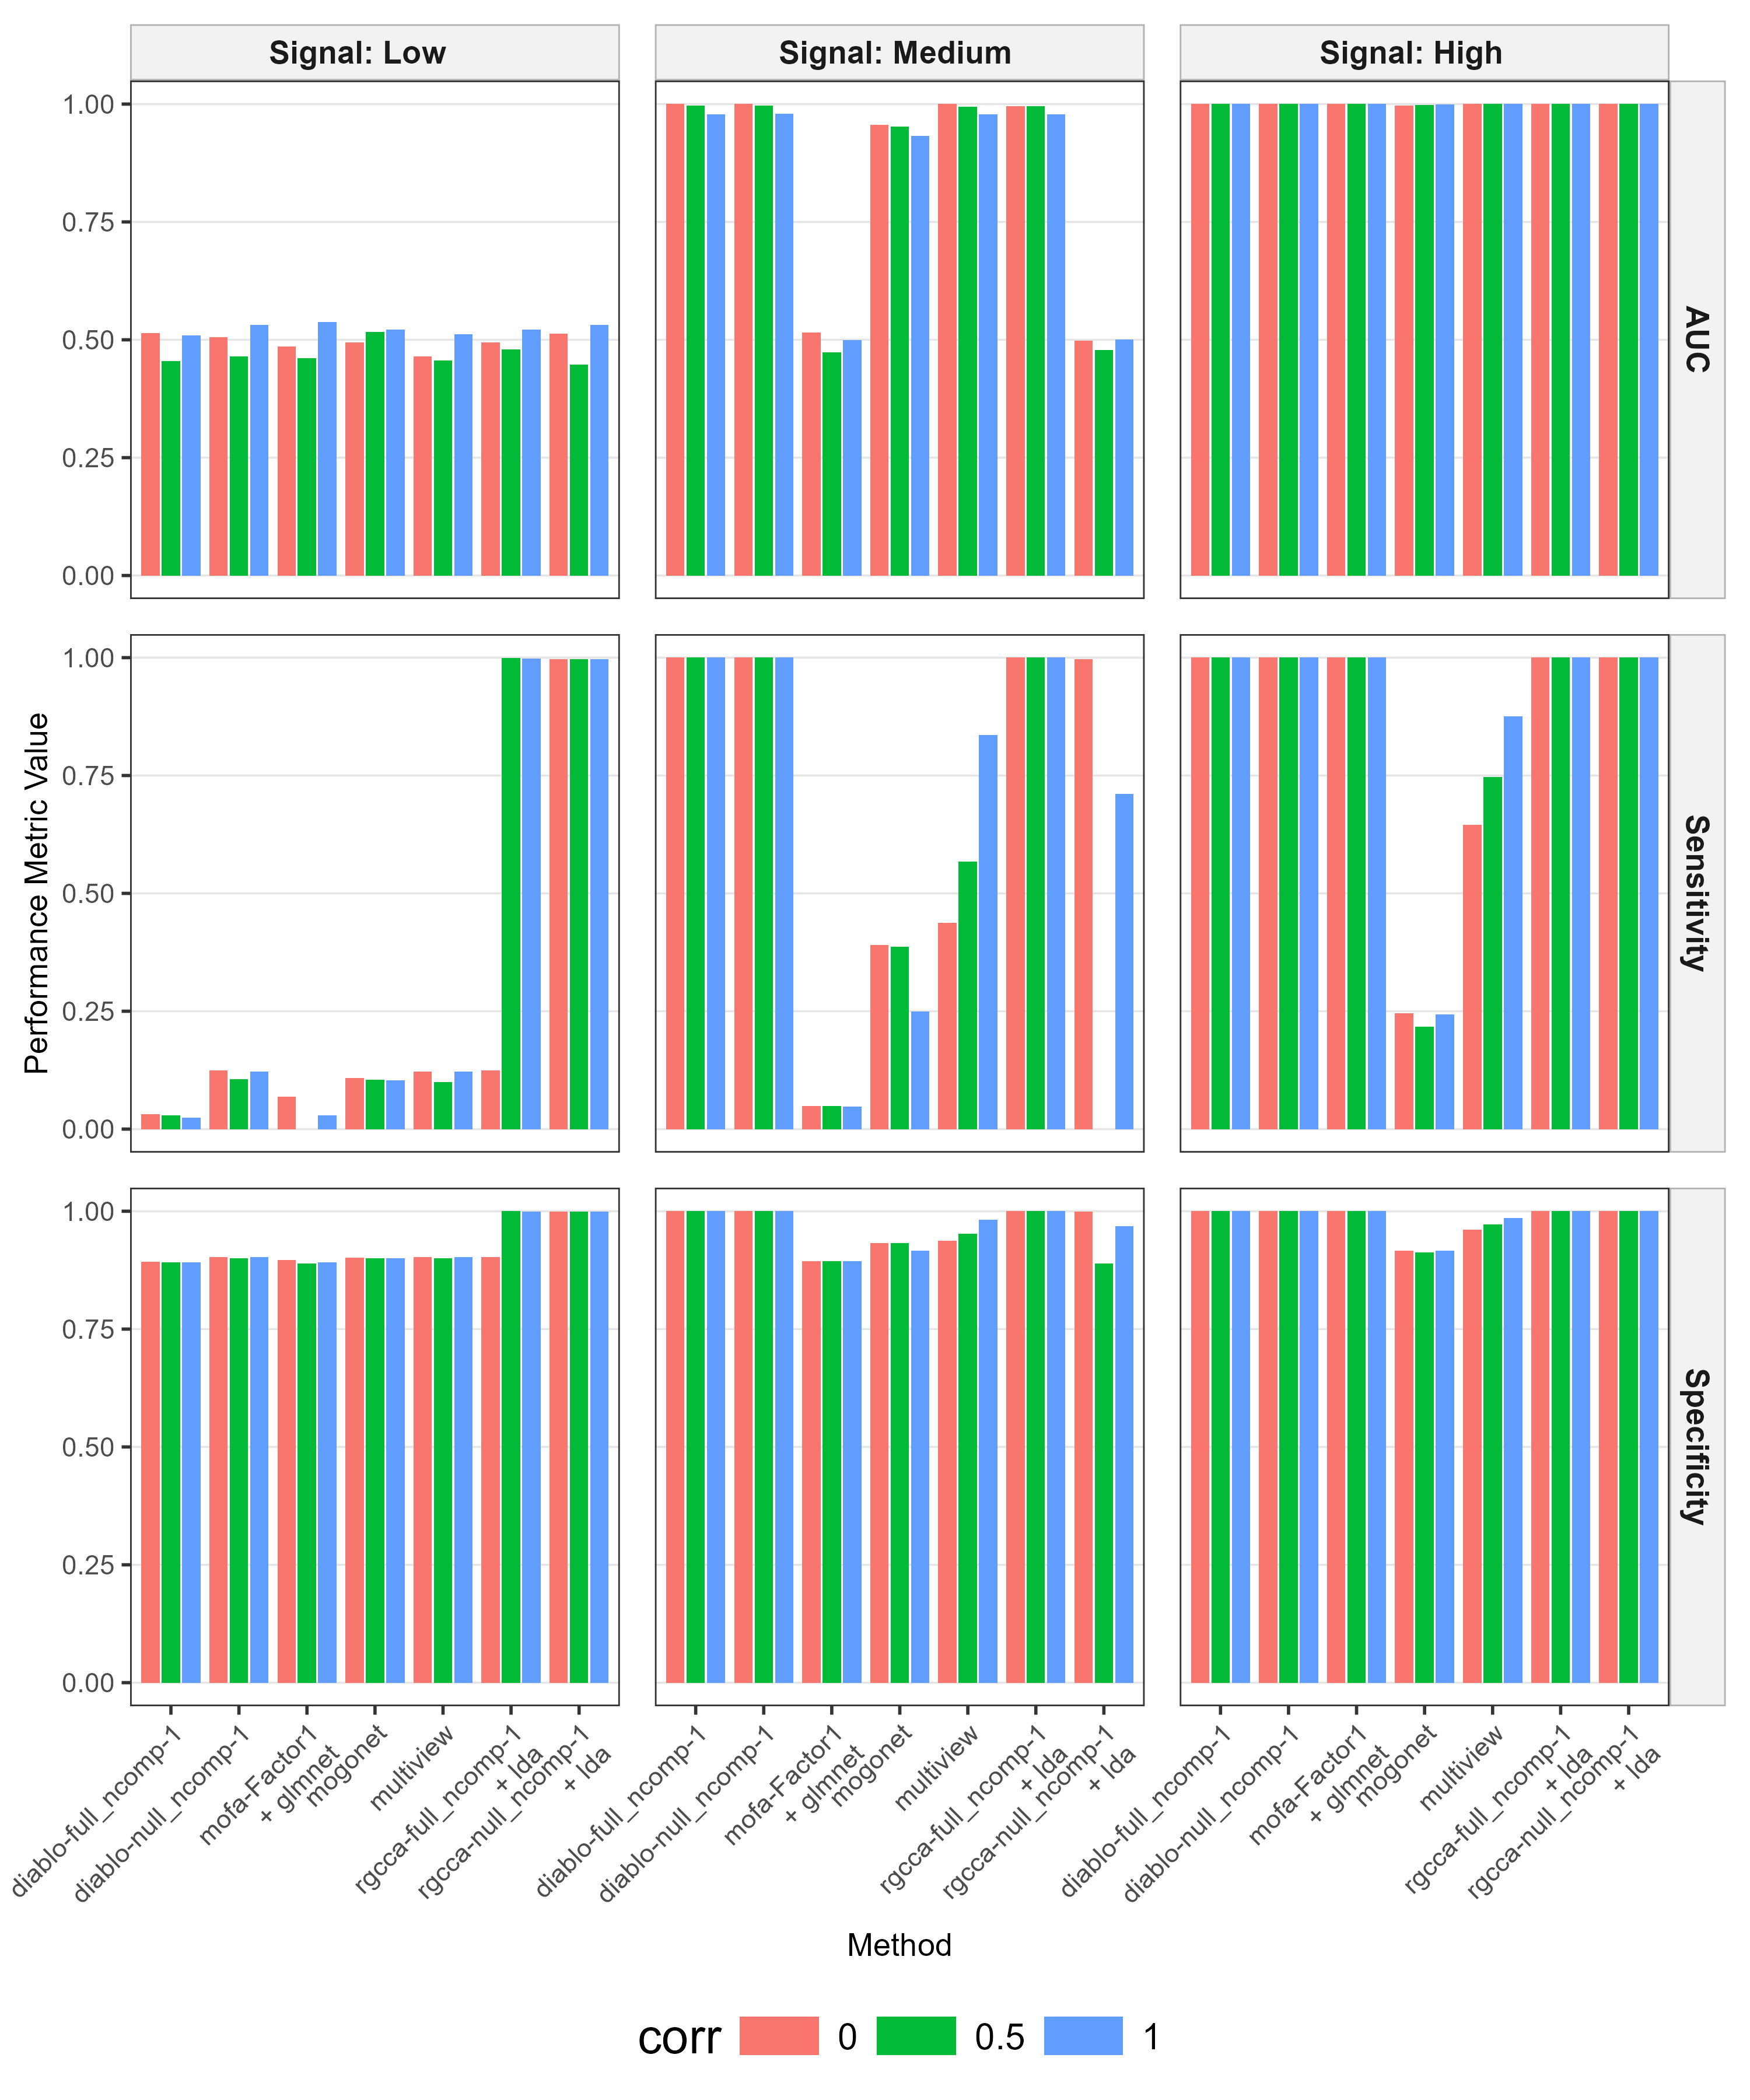
\includegraphics[width=0.96\linewidth]{../results/figures/fig_simulated_performance_grid} 

}

\caption{Simulation studies performances on AUC and feature selection sensitivity/specificity  with varied signal and correlation in the data. Each grid is combination of amount of signal to differentiate response variable classes, and correlation of omics within one complete set of multiomics simulated data. A) Mean Area under the curve (AUC) score of a 5-fold CV. This measures ability of method predictive performance on the response variable, the closer score to 1 (max) is better. B) The sensititivity here is to measure how good methods are identifying the actual signal variables given noise in other variables. The specificity here is to measure how good methods are detecting the noises out. The values of signal are the following: 0, 3, 100 (None, Low, High). The values of correlation are the following: 0, 0.5, 1 (Low, Medium, High)}\label{fig:sim-grid-plot}
\end{figure}

We noticed that as signal increases, method tend to perform better, ultimately its AUC score plateaus at 1 as illustrated in Fig \ref{fig:sim-grid-plot} \textbf{A}. This is expected, as more clear pattern exist in different groups (i.e.~positive vs negative), labels are more distinguished for methods to learn. On the other hand, we also prove that when there's no signal present, method gives a mean AUC of 0.5 , which means it turns out to be randomly guessing the response. This result is also trivial, as there's not clear difference between groups, hence hard to distinguish and models struggle to learn anything meaningful.

With these simple facts, we have showed that simulations are setup correctly, and verified how machine learning works with labelled data.
Furthermore, we noticed that method given little signal, i.e.~\(\text{signal} = 3 > 0\), they all start to work well, quickly bumping its \(0.5\) AUC to \(0.7\) with the exception of mofa-Factor1 and rgcca-null\_ncomp-1.

This have showed data with little variation provided it is clear difference among groups, current SOTA methods are capable to make reasonably well predictions.
We also tested against varying correlation in the omics within each dataset. But, the role of correlation in this simulation is not depicted clearly and requires further understanding and exploration.

In terms of classification performance, DIABLO with different design matrices showed relatively good performance ranking at top. Cooperative Learning follows next with consistent distribution of AUC scores, and less variable compared to other methods. MOFA + glmnet and RGCCA + LDA are in the middle, with high variability. Lastly, MOGONET showed consistenly low performance compared to others and only performing well at no signal and full correlation between omics.

Then from Fig \ref{fig:sim-grid-plot} \textbf{B} we looked at ability and quality of feature selection to identified relevant signal variables or noise variables. Given the large amount of the noise variables in each omics of the data, where only \(300\) of \(3000\) variables in each are actual signal variables. Almost all methods failed at identifying signal variables when low signal. This gets better when increasing amount of signal, yet MOGONET still fails to distinguish signal variables from the noise variables at a signal of \(100\). RGCCA-full-ncomp 1 worked best in different settings of signal followed by DIABLO with null design. On the other hand, all methods due a quite good job in detecting noise variables, this is similar to a classification problem with mostly negative instances.

We believe these sets of simulation studies could be used for future method development, and test them against various scenarios of multiomics data. More parameters could be involved to rigorously test method's robustness. This could be achieved with ease with our proposed pipeline, as we need is to setup the correct data and rest is just handled by these fixed and reproducible workflows.

\hypertarget{model-assessment}{%
\subsection{Model Assessment}\label{model-assessment}}

We further extended the pipeline usage to real-world dataset, such that it could
demonstrate the utility of our pipeline and to comprehensively assess the performance of integration methods. We benchmarked the methods on \(13\) real-world datasets collected from publicly available sources such as the Gene Expression Omnibus (GEO) {[}cite here{]} and The Cancer Genome Atlas (TCGA) {[}cite here{]}, as summarized in Table \ref{tab:benchmark-data-table}.

\begingroup\fontsize{7}{9}\selectfont

\begin{longtable}[t]{>{\raggedright\arraybackslash}p{0.75in}r>{\raggedright\arraybackslash}p{0.7in}>{\raggedright\arraybackslash}p{0.7in}rlrl}
\caption{\label{tab:benchmark-data-table}Overview of real datasets to benchmark}\\
\toprule
Disease & N & Y=0 & Y=1 & Prop(Y = 1) & Omic & P & Dataset\\
\midrule
\endfirsthead
\caption[]{\label{tab:benchmark-data-table}Overview of real datasets to benchmark \textit{(continued)}}\\
\toprule
Disease & N & Y=0 & Y=1 & Prop(Y = 1) & Omic & P & Dataset\\
\midrule
\endhead

\endfoot
\bottomrule
\endlastfoot
 &  &  &  &  & mrna & 8110 & \\

 &  &  &  &  & cpg & 1674 & \\

\multirow[b]{-3}{0.75in}{\raggedright\arraybackslash Autism} & \multirow[b]{-3}{*}{\raggedleft\arraybackslash 24} & \multirow[b]{-3}{0.7in}{\raggedright\arraybackslash control Cer} & \multirow[b]{-3}{0.7in}{\raggedright\arraybackslash autistic} & \multirow[b]{-3}{*}{\raggedleft\arraybackslash 0.458} & cc & 12 & \multirow[b]{-3}{*}{\raggedright\arraybackslash GSE38609}\\
\cmidrule{1-8}
 &  &  &  &  & cpg & 4796 & \\

 &  &  &  &  & mirna & 175 & \\

 &  &  &  &  & rppa & 42 & \\

\multirow[b]{-4}{0.75in}{\raggedright\arraybackslash Stomach and Esophageal Cancer} & \multirow[b]{-4}{*}{\raggedleft\arraybackslash 25} & \multirow[b]{-4}{0.7in}{\raggedright\arraybackslash stagei/stageii} & \multirow[b]{-4}{0.7in}{\raggedright\arraybackslash stageiii/stageiv} & \multirow[b]{-4}{*}{\raggedleft\arraybackslash 0.600} &  & 5590 & \multirow[b]{-4}{*}{\raggedright\arraybackslash TCGA-STES}\\
\cmidrule{1-5}
\cmidrule{7-8}
 &  &  &  &  & \multirow[b]{-2}{*}{\raggedright\arraybackslash mrna} & 5831 & \\

 &  &  &  &  & cpg & 8915 & \\

\multirow[b]{-3}{0.75in}{\raggedright\arraybackslash Bladder Cancer} & \multirow[b]{-3}{*}{\raggedleft\arraybackslash 33} & \multirow[b]{-3}{0.7in}{\raggedright\arraybackslash non-invasive bladder cancer} & \multirow[b]{-3}{0.7in}{\raggedright\arraybackslash invasive bladder cancer} & \multirow[b]{-3}{*}{\raggedleft\arraybackslash 0.424} & cc & 10 & \multirow[b]{-3}{*}{\raggedright\arraybackslash GSE71669}\\
\cmidrule{1-8}
 &  &  &  &  & cpg & 7396 & \\

 &  &  &  &  & mirna & 166 & \\

 &  &  &  &  & rppa & 40 & \\

\multirow[b]{-4}{0.75in}{\raggedright\arraybackslash Adrenocortical Cancer} & \multirow[b]{-4}{*}{\raggedleft\arraybackslash 46} &  &  & \multirow[b]{-4}{*}{\raggedleft\arraybackslash 0.391} & mrna & 5660 & \multirow[b]{-4}{*}{\raggedright\arraybackslash TCGA-ACC}\\
\cmidrule{1-2}
\cmidrule{5-8}
 &  &  &  &  & cpg & 6489 & \\

 &  &  &  &  & mirna & 180 & \\

 &  &  &  &  & rppa & 57 & \\

\multirow[b]{-4}{0.75in}{\raggedright\arraybackslash Adenomas and Adenocarcinomas} &  &  &  & \multirow[b]{-4}{*}{\raggedleft\arraybackslash 0.302} & mrna & 5517 & \multirow[b]{-4}{*}{\raggedright\arraybackslash TCGA-KICH}\\
\cmidrule{1-1}
\cmidrule{5-8}
 &  &  &  &  & cpg & 7647 & \\

 &  &  &  &  & mirna & 203 & \\

 &  &  &  &  & rppa & 41 & \\

\multirow[b]{-4}{0.75in}{\raggedright\arraybackslash Mesothelioma} & \multirow[b]{-8}{*}{\raggedleft\arraybackslash 63} &  &  & \multirow[b]{-4}{*}{\raggedleft\arraybackslash 0.762} & mrna & 5852 & \multirow[b]{-4}{*}{\raggedright\arraybackslash TCGA-MESO}\\
\cmidrule{1-2}
\cmidrule{5-8}
 &  &  &  &  & cpg & 7534 & \\

 &  &  &  &  & mirna & 218 & \\

 &  &  &  &  & rppa & 47 & \\

\multirow[b]{-4}{0.75in}{\raggedright\arraybackslash Skin Cutaneous Cancer} & \multirow[b]{-4}{*}{\raggedleft\arraybackslash 80} &  &  & \multirow[b]{-4}{*}{\raggedleft\arraybackslash 0.350} & mrna & 5691 & \multirow[b]{-4}{*}{\raggedright\arraybackslash TCGA-SKCM}\\
\cmidrule{1-2}
\cmidrule{5-8}
 &  &  &  &  & cpg & 7985 & \\

 &  &  &  &  & mirna & 251 & \\

 &  &  &  &  & rppa & 43 & \\

\multirow[b]{-4}{0.75in}{\raggedright\arraybackslash Breast Invasive Cancer} & \multirow[b]{-4}{*}{\raggedleft\arraybackslash 109} &  &  & \multirow[b]{-4}{*}{\raggedleft\arraybackslash 0.358} & mrna & 5936 & \multirow[b]{-4}{*}{\raggedright\arraybackslash TCGA-BRCA}\\
\cmidrule{1-2}
\cmidrule{5-8}
 &  &  &  &  & cpg & 7963 & \\

 &  &  &  &  & mirna & 202 & \\

 &  &  &  &  & rppa & 44 & \\

\multirow[b]{-4}{0.75in}{\raggedright\arraybackslash Esophageal Cancer} & \multirow[b]{-4}{*}{\raggedleft\arraybackslash 119} &  &  & \multirow[b]{-4}{*}{\raggedleft\arraybackslash 0.353} & mrna & 5709 & \multirow[b]{-4}{*}{\raggedright\arraybackslash TCGA-ESCA}\\
\cmidrule{1-2}
\cmidrule{5-8}
 &  &  &  &  & cpg & 7726 & \\

 &  &  &  &  & mirna & 214 & \\

 &  &  &  &  & rppa & 44 & \\

\multirow[b]{-4}{0.75in}{\raggedright\arraybackslash Kidney Cancer} & \multirow[b]{-4}{*}{\raggedleft\arraybackslash 123} &  &  & \multirow[b]{-4}{*}{\raggedleft\arraybackslash 0.520} & mrna & 5941 & \multirow[b]{-4}{*}{\raggedright\arraybackslash TCGA-KIRC}\\
\cmidrule{1-2}
\cmidrule{5-8}
 &  &  &  &  & cpg & 6367 & \\

 &  &  &  &  & mirna & 231 & \\

 &  &  &  &  & rppa & 25 & \\

\multirow[b]{-4}{0.75in}{\raggedright\arraybackslash Thyroid Cancer} & \multirow[b]{-4}{*}{\raggedleft\arraybackslash 217} &  &  & \multirow[b]{-4}{*}{\raggedleft\arraybackslash 0.318} & mrna & 5537 & \multirow[b]{-4}{*}{\raggedright\arraybackslash TCGA-THCA}\\
\cmidrule{1-2}
\cmidrule{5-8}
 &  &  &  &  & cpg & 8072 & \\

 &  &  &  &  & mirna & 268 & \\

 &  &  &  &  & rppa & 44 & \\

\multirow[b]{-4}{0.75in}{\raggedright\arraybackslash Bladder Cancer} & \multirow[b]{-4}{*}{\raggedleft\arraybackslash 336} & \multirow[b]{-36}{0.7in}{\raggedright\arraybackslash stagei/stageii} & \multirow[b]{-36}{0.7in}{\raggedright\arraybackslash stageiii/stageiv} & \multirow[b]{-4}{*}{\raggedleft\arraybackslash 0.685} & mrna & 6093 & \multirow[b]{-4}{*}{\raggedright\arraybackslash TCGA-BLCA}\\
\cmidrule{1-8}
 &  &  &  &  & cpg & 58 & \\

 &  &  &  &  & genomics & 74 & \\

\multirow[b]{-3}{0.75in}{\raggedright\arraybackslash Alzheimer's Disease} & \multirow[b]{-3}{*}{\raggedleft\arraybackslash 351} & \multirow[b]{-3}{0.7in}{\raggedright\arraybackslash normal control} & \multirow[b]{-3}{0.7in}{\raggedright\arraybackslash alzheimer's disease} & \multirow[b]{-3}{*}{\raggedleft\arraybackslash 0.519} & mrna & 90 & \multirow[b]{-3}{*}{\raggedright\arraybackslash ROSMAP}\\*
\end{longtable}
\endgroup{}

In the meantime, we have benchmarked \(5\) methods: DIABLO (\protect\hyperlink{ref-singh2019diablo}{Singh \emph{et al.}, 2019}), Cooperative Learning (\protect\hyperlink{ref-ding2022cooperative}{Ding \emph{et al.}, 2022}), MOGONET (\protect\hyperlink{ref-wang2021mogonet}{Wang \emph{et al.}, 2021}), RGCCA (\protect\hyperlink{ref-girka2023multiblock}{Girka \emph{et al.}, 2023}), MOFA (\protect\hyperlink{ref-Argelaguet2018}{Argelaguet \emph{et al.}, 2018}, \protect\hyperlink{ref-Argelaguet2020}{2020}). Additional candidate methods and implementation options available through the pipeline are listed in Table \ref{tab:method-meta-table}.

To start, we measured the computational cost of each method in terms of runtime and memory usage. This included the total runtime and memory usage across key stages of the pipeline: input preprocessing, model training, prediction, and feature selection. These resource metrics allow for a holistic comparison of methods in terms of both performance and computational efficiency.

Then, we evaluated classification performance using standard binary classification metrics: area under the receiver operating characteristic curve (AUC), balanced accuracy, and F1 score, computed using 5-fold cross-validation. The full cross-validation procedure and metric definitions are detailed in the \protect\hyperlink{methods}{Methods} section. This allowed us to compare each method's predictive performance across all datasets in a consistent manner.

Due to the fact of ground truth of real datasets are not available, the interpretation of the feature selection part is different than the simulation studies. Hence, we have extracted features importances and run it against a Gene Set Enrichment Analysis (GSEA) {[}cite here{]} under two public source pathway databases like KEGG {[}cite here{]} and PanglaoDB {[}cite here{]} to see its biological relevance.

\hypertarget{computational-resourcs-usage}{%
\subsubsection{Computational Resourcs Usage}\label{computational-resourcs-usage}}

The benchmarking results highlight substantial variation in both runtime duration and memory usage across multiview learning methods and computational stages.

\begin{figure}

{\centering \includegraphics[width=0.96\linewidth]{../results/figures/fig_computational_resources_usage} 

}

\caption{Mean runtime and memory usage of methods across computational stages.(A) Duration (in seconds, log10 scale) of each method separated by stage: preprocessing, model training, prediction, and feature selection. (B) Corresponding RAM memory usage (in megabytes, log10 scale) for the same stages. Bars represent mean values with error bars indicating standard deviations. Each stage is color-coded: preprocessing (yellow), training (blue), prediction (green), and feature selection (pink).}\label{fig:computational-resource-plot}
\end{figure}

As shown in (Fig \ref{fig:computational-resource-plot} panel A), model training is consistently the most time-consuming step across all methods, with MULTIVIEW and MOGONET requiring notably longer durations compared to RGCCA, MOFA, and DIABLO. Despite the high training time of MULTIVIEW, its prediction stage is relatively efficient and on par with other methods. Preprocessing time remains consistent across methods, suggesting similar data preparation pipelines or overheads. Feature selection duration shows more variability, with MULTIVIEW again standing out as the most computationally expensive, while DIABLO and MOFA appear to be the most efficient overall.

In terms of RAM usage (Fig \ref{fig:computational-resource-plot} panel B), similar trends are observed. Model training and prediction steps tend to demand more memory than preprocessing or feature selection, particularly for MULTIVIEW and MOGONET, which consume the most memory during prediction. This is likely due to the complexity of their underlying architectures or model size. Interestingly, DIABLO and MOFA show efficient memory use across all stages, indicating their suitability for resource-constrained environments. The consistently higher memory demand during the prediction phase for MULTIVIEW raises practical concerns for deployment, especially in real-time or large-scale applications. Overall, while MULTIVIEW and MOGONET may offer modeling advantages, they do so at the cost of higher computational resource requirements.

\hypertarget{real-dataset-classification-performances}{%
\subsubsection{Real dataset classification performances}\label{real-dataset-classification-performances}}

After evaluating the pipeline with simulation studies, we then proceed to execute it with real world datasets as describe in table \ref{tab:benchmark-data-table}. The scripts to clean these data could be found under {[}insert link here\ldots{]}.

We noticed the AUC scores follows a similar pattern from the simulations, where most of the AUC fall around \(0.7\) as per Fig \ref{fig:real-perf-plot}, this is exactly the case when we have little signal in the data.
These real datasets that we evaluated are mostly carnicoma cohorts from TCGA, where usually we have fewer observations in later stage carnicoma, and its molecular measurement are not much different with those early stage, i.e.~stageii vs stageiii. Furthermore, we have datasets that have near \(0.5\), this could indicate low signal present in those datasets.

In terms of performance ranking, DIABLO still perform at top compared to other methods, where its variant with null design matrix beats performance with full design matrix. This design matrix represents connection or correlation between the omics inside the data. Similar to our simulations, Cooperative Learning follows after DIABLO. Although this time, there are competitions between rest models where all perform moderately. Arguably, one of MOFA + glmnet or MOGONET perform as weakest.

From here, we verified that there's no such method that could perform well in all possible scenarios, it could be top in certain dataset, but it could also be weakest in some specific dataset, i.e Cooperative Learning has best overall high AUC, but it struglles particularly in the TCGA-STES dataset that studies stomach and esophageal carcinoma. This might be due to the limited sample size of this dataset with only \(25\) observations.
Therefore, we prove the pipeline provides an easy way to benchmark multiomics integration methods in purely data-driven approach, and could quickly compare large set of methods at once, and targeting possible candidate method that suits user custom data the most. This way, researcher won't have to figure out setting environments to test certain method against their data, and save their time by fitering out methods that are not best suit to their needs.

\begin{figure}

{\centering 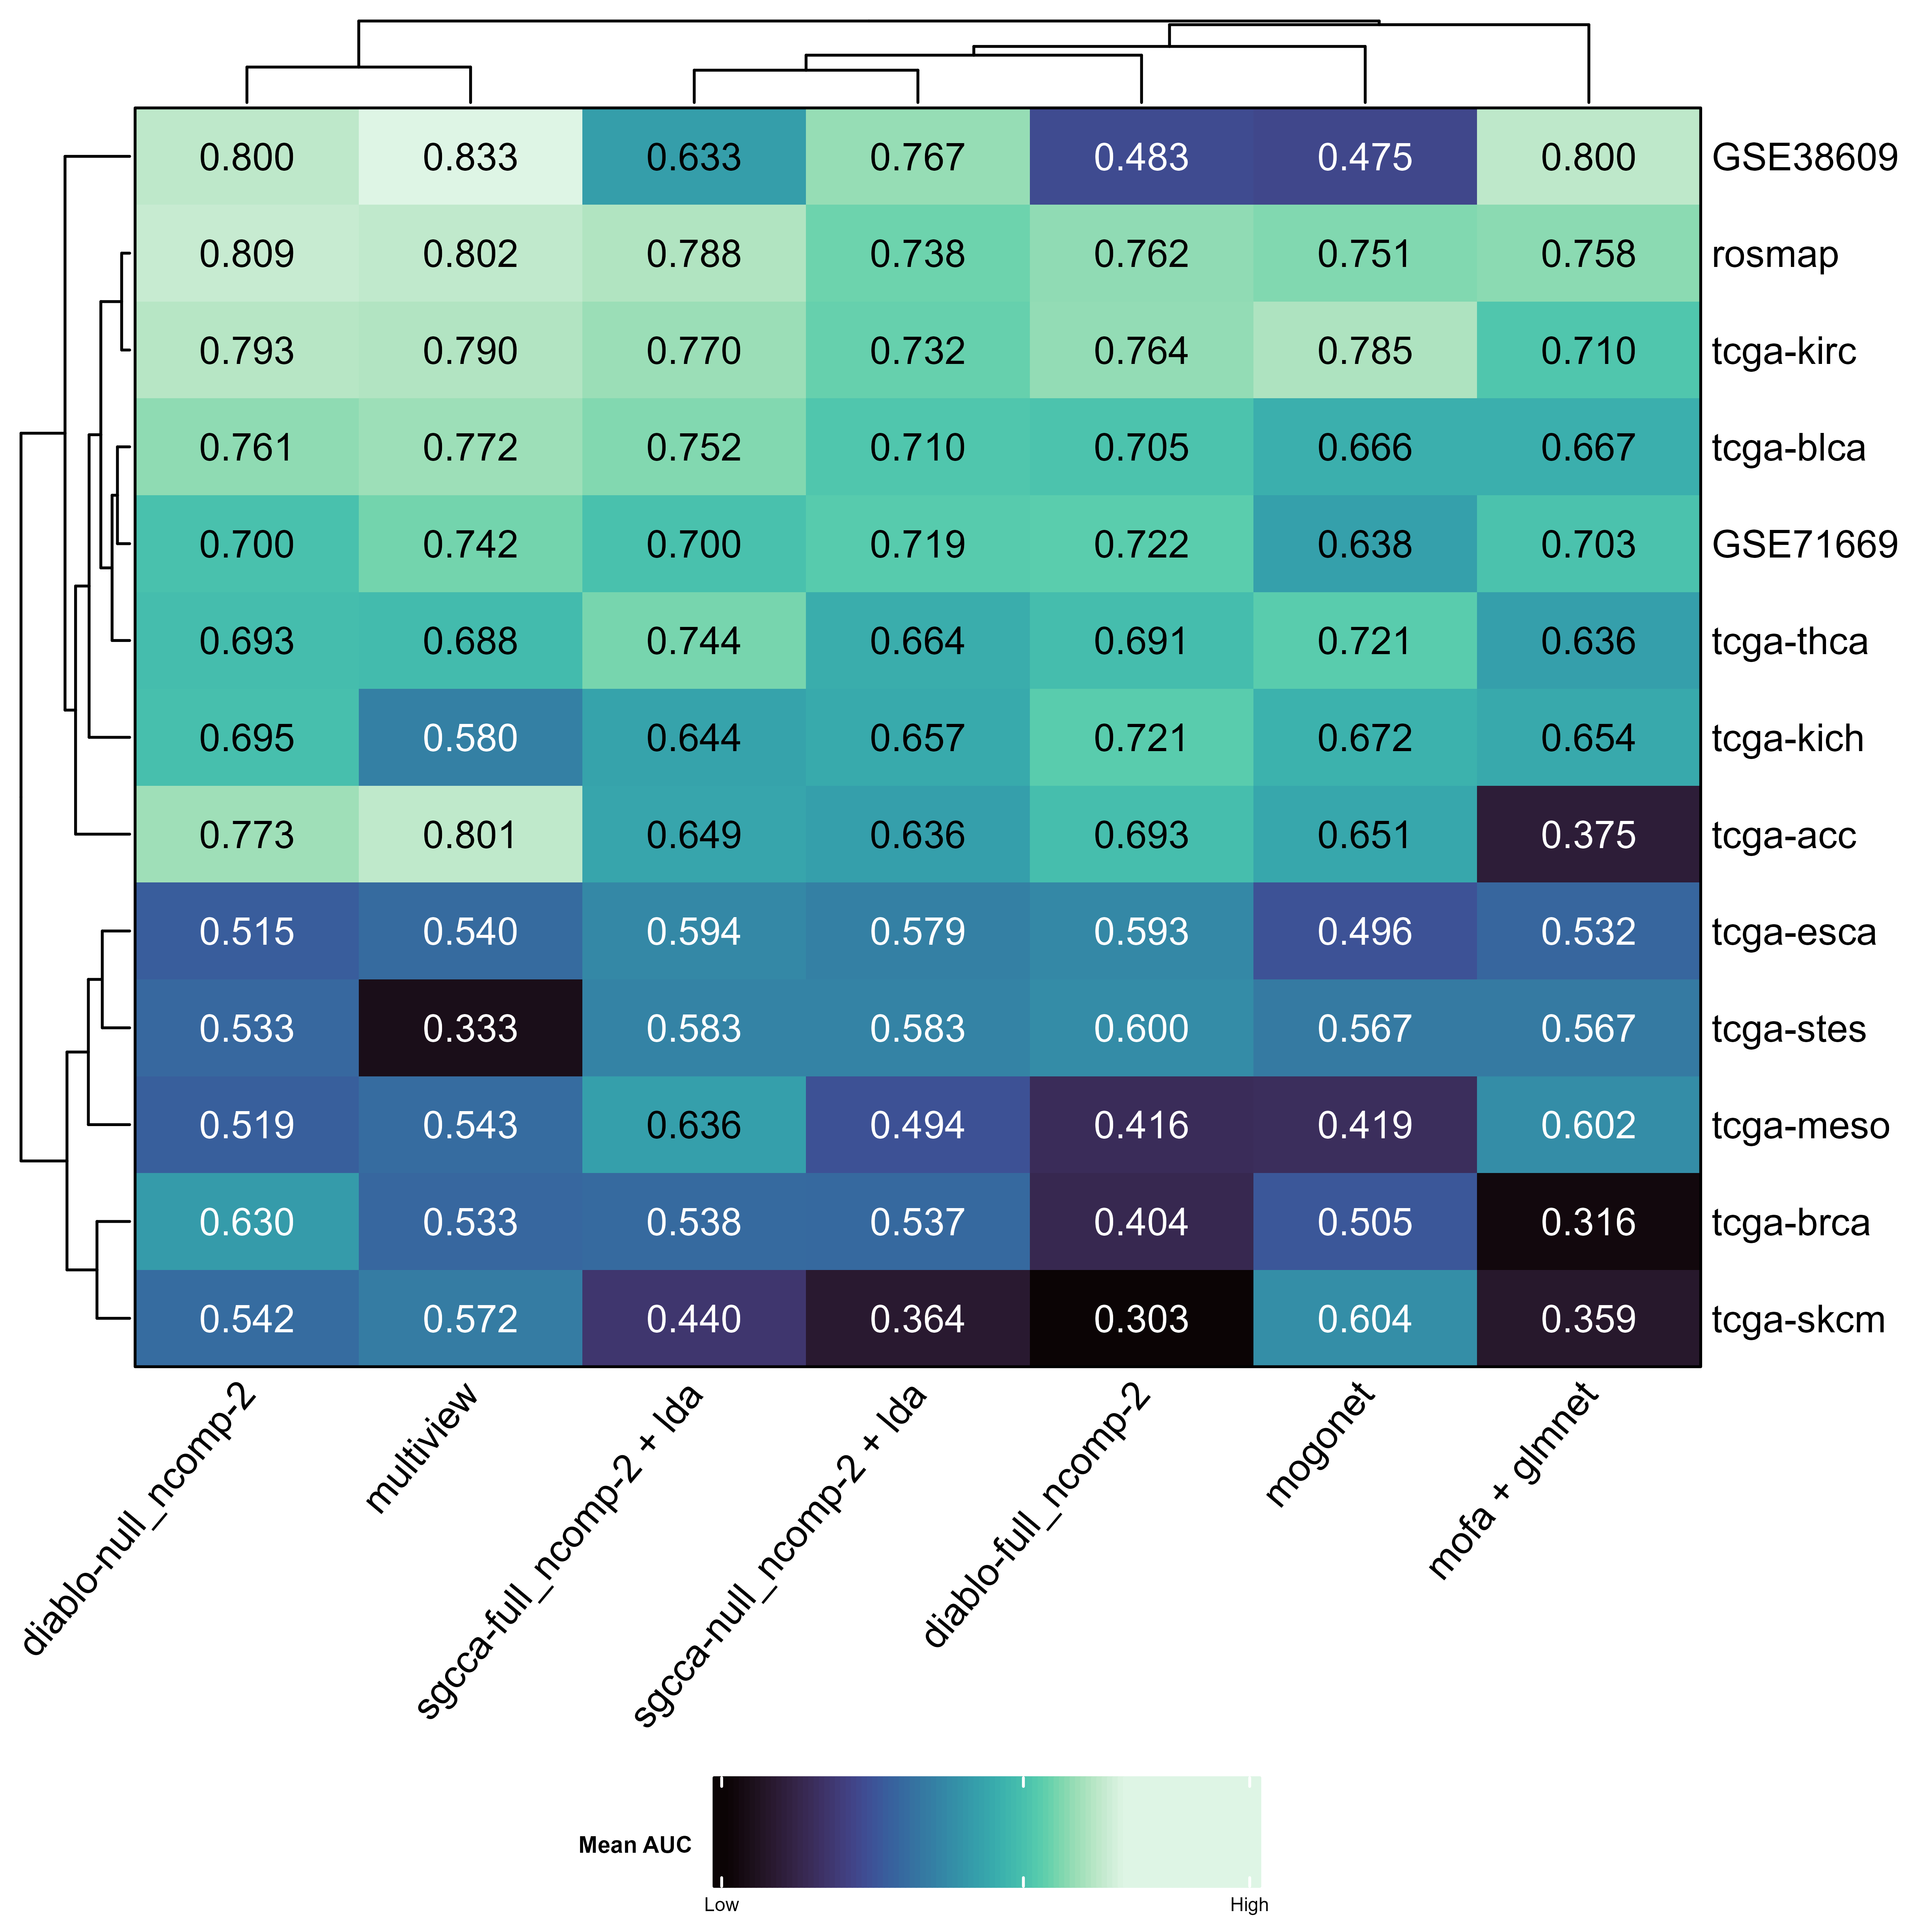
\includegraphics[width=0.96\linewidth]{../results/figures/fig_performance_evaluation_real} 

}

\caption{Heatmap of mean AUC from 5 fold-CV. This heatmap represents the mean area under the curve score taken from a 5 fold cross validation evaluated for each method + dataset combination. Lighter color indicates better score or performance of the method. A mean AUC score > 0.7 is considered good. Dendograms indicates possibble relationship between two columns/rows. DIABLO, RGCCA and MOFA are fitting 2 components.}\label{fig:real-perf-plot}
\end{figure}

\hypertarget{biological-relevance-interpretation}{%
\subsubsection{Biological Relevance Interpretation}\label{biological-relevance-interpretation}}

To enhance biological relevance of these datasets, we examined FGSEA {[}insert citation{]} on all the datasets + method combination separately after the pipeline at Fig
\ref{fig:fgsea-analysis-plot}

\begin{figure}

{\centering 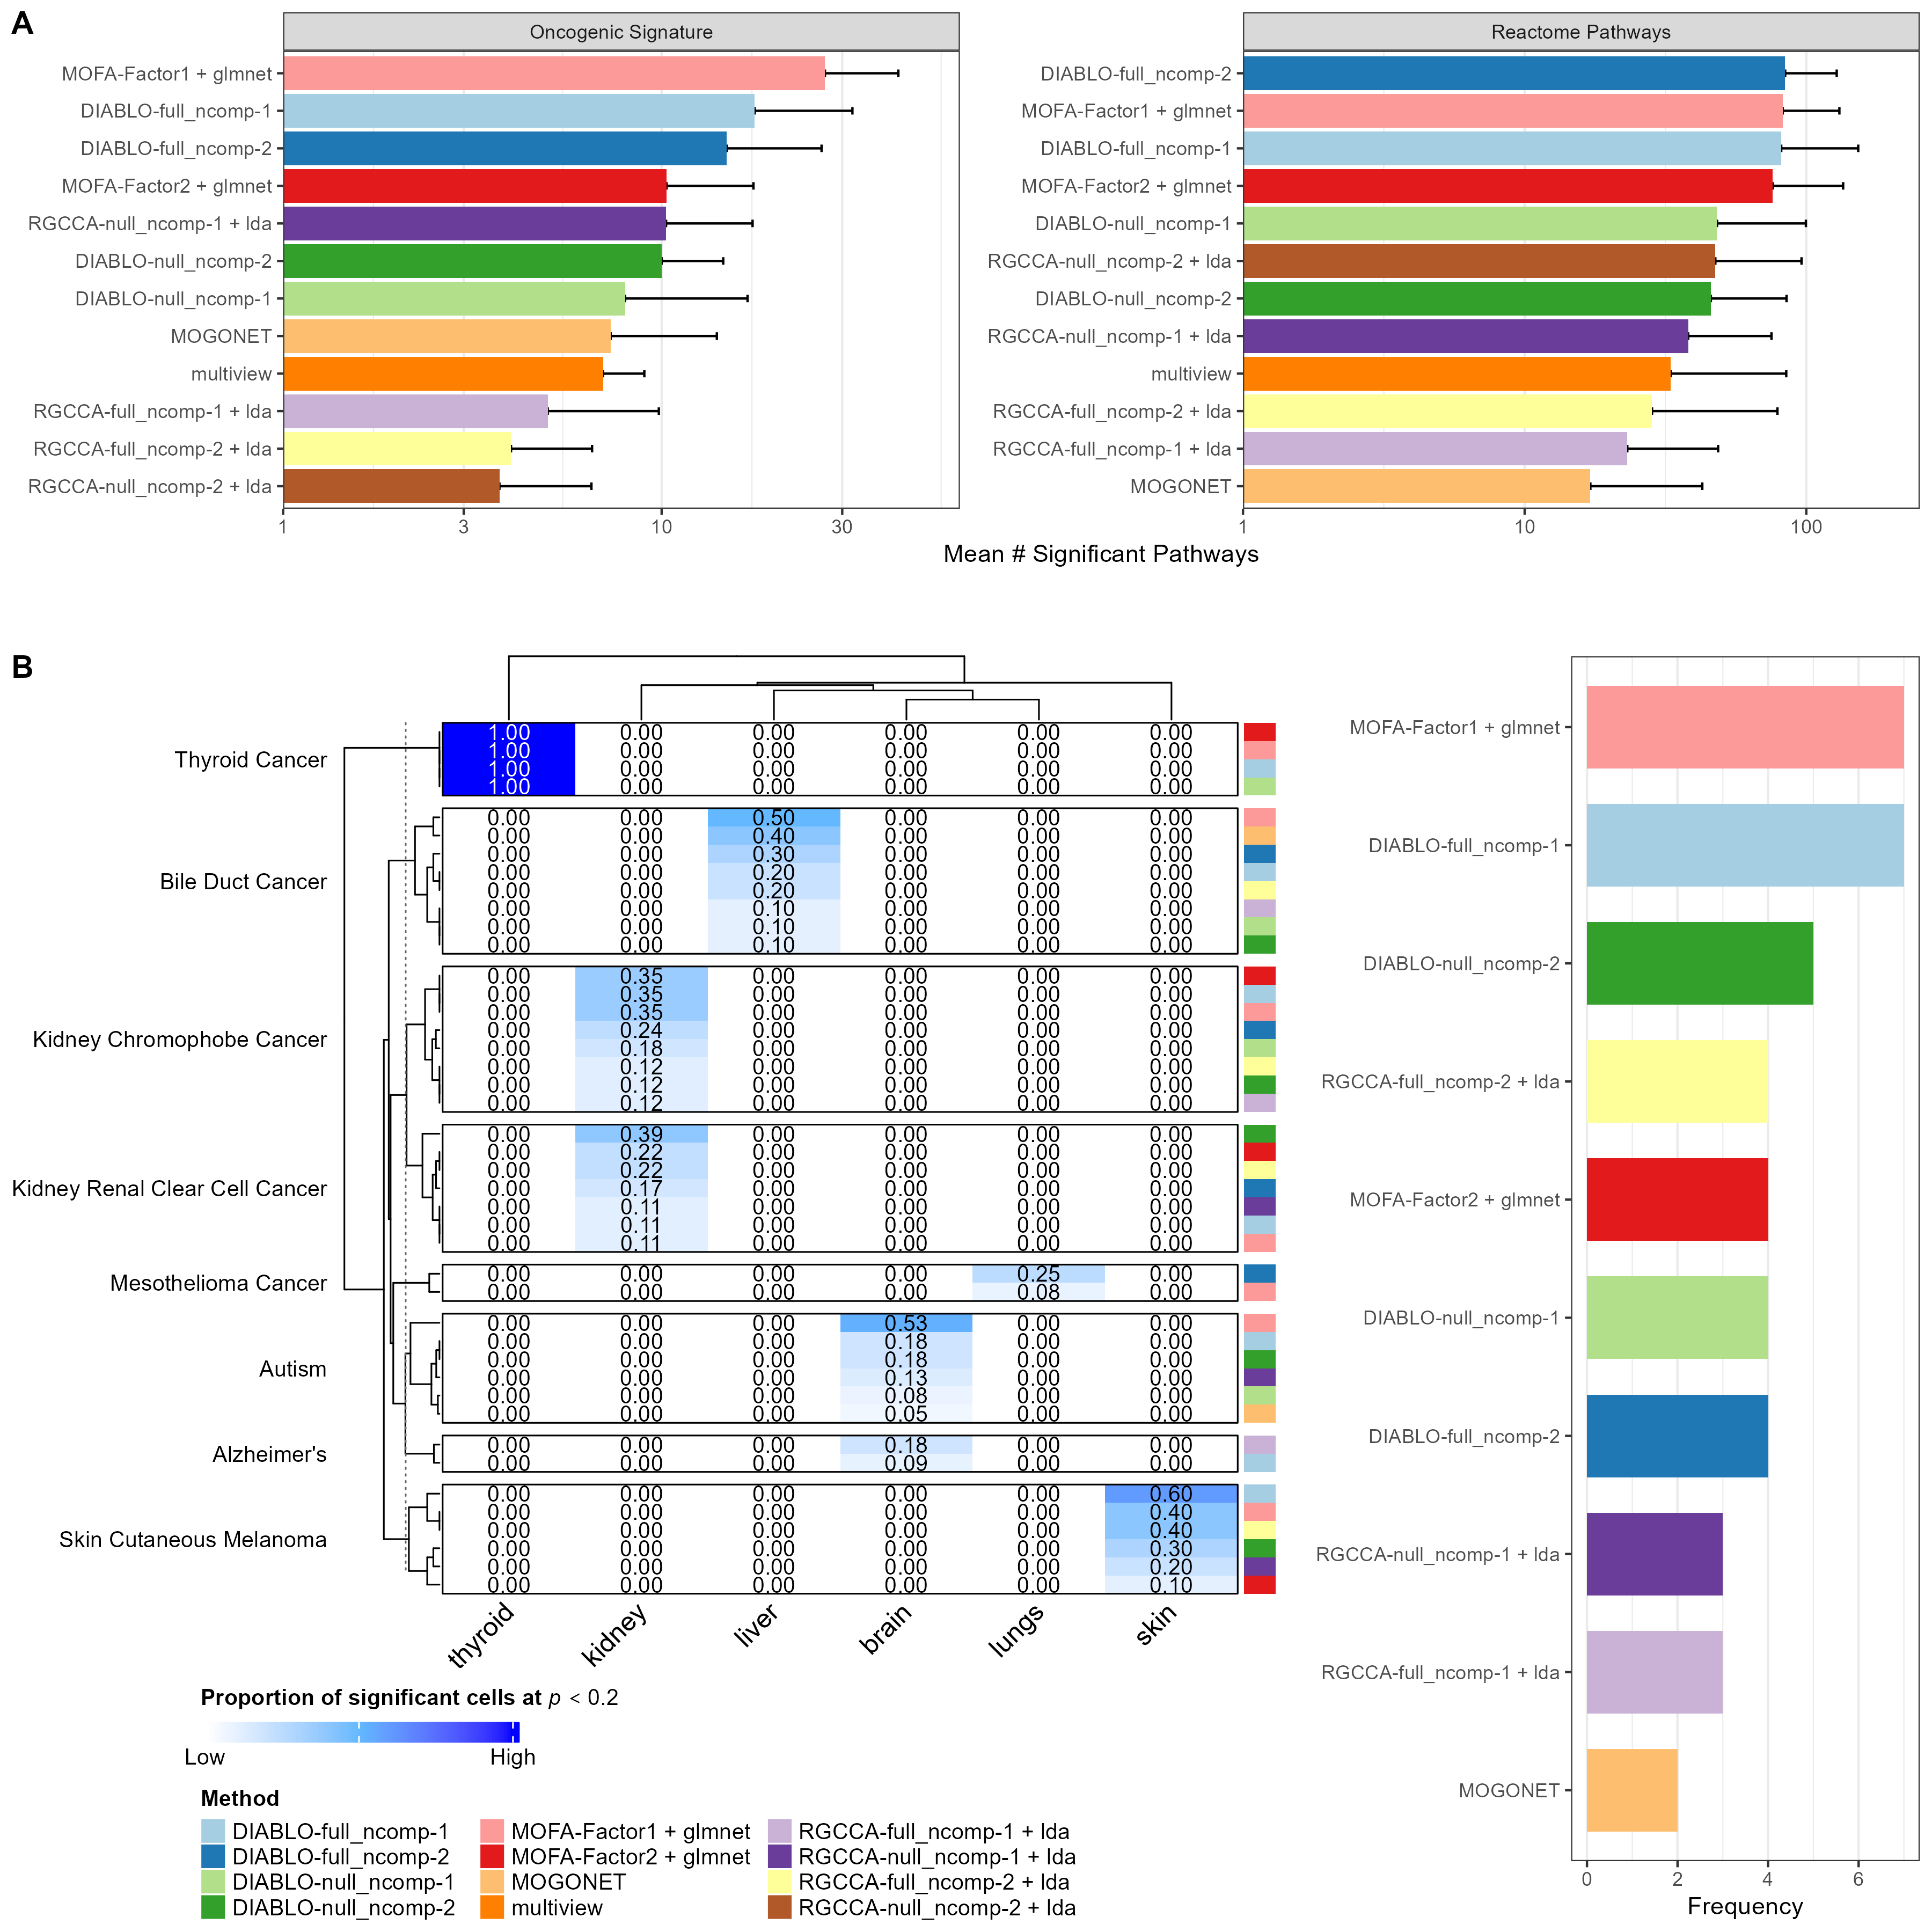
\includegraphics[width=0.92\linewidth]{../results/figures/fig_fgsea_analysis_two_panels} 

}

\caption{Comparative evaluation of multiomics integration methods for identifying significant pathways through gene set enrichment analysis. (A) Mean number of significant pathways detected across methods for two pathway databases: Oncogenic Signature (left) and Reactome (right), with error bars indicating variability. (B) Heatmap showing the proportion of significant pathway–tissue–disease associations (cells) for each method across multiple disease types and tissues. Blue intensity reflects a higher proportion of significant results. The side barplot on the right summarizes the frequency each method appears among the top performers for each tissue–disease pair.}\label{fig:fgsea-analysis-plot}
\end{figure}

This analysis demonstrates the relative effectiveness of different multiomics methods in identifying known pathway associations across diseases. In panel A, MOGONET achieved the highest mean number of significant pathways in the Oncogenic Signature database, while diablo-full-ncomp-1 and mofa-factor2 + glmnet consistently identified more significant Reactome pathways.

Panel B highlights disease and tissue specific strengths of each method. For example, mofa-factor1 + glmnet and diablo-full-ncomp-1 are particularly effective for Thyroid Cancer and Melanoma. The horizontal barplot shows that mofa-factor1 + glment and diablo-full-ncomp-1 are most frequently top performers across diseases and tissues.

Overall, these results suggest that while some methods are more generalizable across datasets (e.g., diablo-full-ncomp-1), others may perform better in specific biological contexts. This has implications for selecting appropriate methods based on the disease or tissue of interest.

\hypertarget{discussion}{%
\section{Discussion}\label{discussion}}

\begin{itemize}
\tightlist
\item
  Explain results, and relevant comments to these
\end{itemize}

\hypertarget{conclusion}{%
\section{Conclusion}\label{conclusion}}

Overall, DIABLO emerged as the top performer in terms of classification performance, with relatively consistent computational time Conversely, MOGONET, leveraging deep neural networks, displayed the weakest performance. While acknowledging the potential for further enhancements through exploration of additional datasets and methodologies, we encountered a significant challenge of no publicly available repository/data portal with curated multiomics data.

To address this gap, we have begun to curate multiomics studies for various omics data (e.g., transcriptomics, methylation, proteomics) and associated clinical metadata across a range of cancer and non-cancer diseases from various public sources to create the first data portal for multiomics data (\textasciitilde{} 100 studies) in both standard formats mentioned such that they can easily be used by other researchers.

We anticipate this exercise to be highly relevant to the community utilizing multiomics data for their research, such will help inform the development of a new integrative method that is applicable to different types (bulk, single-cell, or spatial) of multiomics data.

Lastly, due to the modularity of our pipeline, any additional method or dataset could be easily added, and used to compare with existing methods implemented inside the pipeline

\newpage

\hypertarget{methods}{%
\section{Methods}\label{methods}}

\hypertarget{dataset}{%
\subsection{Dataset}\label{dataset}}

We consider multiomics dataset represented by \(P\) omics matrices \(X_i\) , where \(X_i\) is of dimension \(n \times p_i\) (\(n\) samples and \(p_i\) features) for \(i = 1, \dots, P\).

The real dataset were retrieved from public sources like TCGA \href{citation}{{[}citation here{]}} \href{citation}{{[}citaiton here{]}} with R 4.3.3 and libraries TCGAbiolinks 2.30.4 and GEOquery 2.70.0.
These dataset were furthered processed to keep matched samples data only (same subjects measured in different omics modalities)
Furthermore, they are filtered for omics with non zero variance during the pipeline execution, as certain methods would not work if zero variance data was present.
For a summarized list of real dataset, please refer to table \href{cite}{{[}cite the dataset table{]}}. Below we present higher level information of dataset studied in this paper.

\hypertarget{gse38609}{%
\subsubsection{GSE38609}\label{gse38609}}

This data is retrieved from \url{https://www.ncbi.nlm.nih.gov/geo/query/acc.cgi?acc=GSE38609} with title: \emph{Brain transcriptional and epigenetic associations with the autistic phenotype}. It is composed of an expression data with Illumina HumanHT-12 V4.0 expression beadchip and methylation data with Illumina HumanMethylation27 BeadChip. 24 of the original 72 samples are kept after preprocessing in R 4.2 under our pipeline.

\hypertarget{tcga-stes}{%
\subsubsection{TCGA-STES}\label{tcga-stes}}

This data is retrieved from \url{https://www.linkedomics.org/data_download/TCGA-STES/}, and studies \emph{Stomach and Esophageal carcinoma} (STES). It is made of methylation data of Illumina HM450K platform, miRNA data of Illumina HiSeq platform, miRgene-level with RPM normalization, reverse phase protein array (RPPA) gene level data, and RNAseq data normalized counts (Illumina HiSeq platform, Gene-level, RPKM). 25 of the original 625 samples are kept after preprocessing in R 4.2 under our pipeline.

\hypertarget{tcga-chol}{%
\subsubsection{TCGA-CHOL}\label{tcga-chol}}

This data is retrieved from \url{https://www.linkedomics.org/data_download/TCGA-CHOL/}, and studies \emph{Cholangiocarcinoma} or commonly known as bile duct cancer. It is composed of an miRNA with RPM normalization, methylation data with Illumina HM450K platform, RPPA data, and RNAseq data normalized counts (Illumina HiSeq platform, Gene-level, RPKM). 30 of the original 45 samples are kept after preprocessing in R 4.2 under our pipeline.

\hypertarget{gse71669}{%
\subsubsection{GSE71669}\label{gse71669}}

This data is retrieved from \url{https://www.ncbi.nlm.nih.gov/geo/query/acc.cgi?acc=GSE71669} with title: \emph{Integration analysis of three omics data using penalized regression methods: An application to bladder cancer}. It is composed of expression data with Affymetrix Human Gene 1.0 ST Array {[}transcript (gene) version{]} and methylation data with Illumina HumanMethylation27 BeadChip (HumanMethylation27\_270596\_v.1.2). 33 of the original 90 samples are kept after preprocessing in R 4.2 under our pipeline.

\hypertarget{tcga-acc}{%
\subsubsection{TCGA-ACC}\label{tcga-acc}}

This data is retrieved from \url{https://www.linkedomics.org/data_download/TCGA-ACC/} and studies \emph{Adrenocortical carcinoma} (ACC). It is composed of methylation data of tumor samples at Gene level from Illumina HM450K platform, miRNA expression for tumor samples with RPM normalization, RPPA expression normalized (Gene-level), and RNAseq data normalized counts (Illumina HiSeq platform, Gene-level, RPKM). 46 of the original 92 samples are kept after preprocessing in R 4.2 under our pipeline.

\hypertarget{tcga-kich}{%
\subsubsection{TCGA-KICH}\label{tcga-kich}}

This data is retrieved from \url{https://www.linkedomics.org/data_download/TCGA-KICH/} and studies \emph{Kidney Chromophobe}. It is composed of methylation data of tumor samples at Gene level from Illumina HM450K platform, miRNA expression for tumor samples with RPM normalization, RPPA expression normalized (Gene-level), and RNAseq data normalized counts (Illumina HiSeq platform, Gene-level, RPKM). 63 of the original 113 samples are kept after preprocessing in R 4.2 under our pipeline.

\hypertarget{tcga-meso}{%
\subsubsection{TCGA-MESO}\label{tcga-meso}}

This data is retrieved from \url{https://www.linkedomics.org/data_download/TCGA-MESO/} and studies \emph{Mesothelioma}. It is composed of methylation data of tumor samples at Gene level from Illumina HM450K platform, miRNA expression for tumor samples with RPM normalization, RPPA expression normalized (Gene-level), and RNAseq data normalized counts (Illumina HiSeq platform, Gene-level, RPKM). 63 of the original 87 samples are kept after preprocessing in R 4.2 under our pipeline.

\hypertarget{tcga-skcm}{%
\subsubsection{TCGA-SKCM}\label{tcga-skcm}}

This data is retrieved from \url{https://www.linkedomics.org/data_download/TCGA-SKCM/} and studies \emph{Skin Cutaneous Melanoma}. It is composed of methylation data of tumor samples at Gene level from Illumina HM450K platform, miRNA expression for tumor samples with RPM normalization, RPPA expression normalized (Gene-level), and RNAseq data normalized counts (Illumina HiSeq platform, Gene-level, RPKM). 80 of the original 470 samples are kept after preprocessing in R 4.2 under our pipeline.

\hypertarget{tcga-brca}{%
\subsubsection{TCGA-BRCA}\label{tcga-brca}}

This data is retrieved from \url{https://www.linkedomics.org/data_download/TCGA-BRCA/} and studies \emph{Breast invasive carcinoma}. It is composed of methylation data of tumor samples at Gene level from Illumina HM450K platform, miRNA expression for tumor samples (Illumina GenomeAnalyzer platform, Normalized, miRgene-level, RPM), RPPA expression normalized (Gene-level), and RNAseq data normalized counts (Illumina HiSeq platform, Gene-level, RPKM). 109 of the original 1097 samples are kept after preprocessing in R 4.2 under our pipeline.

\hypertarget{tcga-esca}{%
\subsubsection{TCGA-ESCA}\label{tcga-esca}}

This data is retrieved from \url{https://www.linkedomics.org/data_download/TCGA-ESCA/} and studies \emph{Esophageal carcinoma}. It is composed of methylation data of tumor samples at Gene level from Illumina HM450K platform, miRNA expression for tumor samples with RPM normalization, RPPA expression normalized (Gene-level), and RNAseq data normalized counts (Illumina HiSeq platform, Gene-level, Normalized log2 RPKM). 119 of the original 185 samples are kept after preprocessing in R 4.2 under our pipeline.

\hypertarget{tcga-kirc}{%
\subsubsection{TCGA-KIRC}\label{tcga-kirc}}

This data is retrieved from \url{https://www.linkedomics.org/data_download/TCGA-KIRC/} and studies \emph{Kidney renal clear cell carcinoma}. It is composed of methylation data of tumor samples at Gene level from Illumina HM450K platform, miRNA expression for tumor samples (Illumina GenomeAnalyzer platform, miRgene-level, Normalized, RPM), RPPA expression normalized (Gene-level), and RNAseq data normalized counts (Illumina HiSeq platform, Gene-level, RPKM). 80 of the original 123 samples are kept after preprocessing in R 4.2 under our pipeline.

\hypertarget{tcga-thca}{%
\subsubsection{TCGA-THCA}\label{tcga-thca}}

This data is retrieved from \url{https://www.linkedomics.org/data_download/TCGA-THCA/} and studies \emph{Thyroid carcinoma}. It is composed of methylation data of tumor samples at Gene level from Illumina HM450K platform, miRNA expression for tumor samples with RPM normalization, RPPA expression normalized (Gene-level). and RNAseq data normalized counts (Illumina HiSeq platform, Gene-level, Normalized log2 RPKM). 217 of the original 503 samples are kept after preprocessing in R 4.2 under our pipeline.

\hypertarget{tcga-blca}{%
\subsubsection{TCGA-BLCA}\label{tcga-blca}}

This data is retrieved from \url{https://www.linkedomics.org/data_download/TCGA-BLCA/} and studies \emph{Bladder urothelial carcinoma}. It is composed of methylation data of tumor samples at Gene level from Illumina HM450K platform, miRNA expression for tumor samples with RPM normalization, RPPA expression normalized (Gene-level), and RNAseq data normalized counts (Illumina HiSeq platform, Gene-level, Normalized log2 RPKM). 336 of the original 412 samples are kept after preprocessing in R 4.2 under our pipeline.

\hypertarget{rosmap}{%
\subsubsection{ROSMAP}\label{rosmap}}

This data is obtained from AMP-AD Knowledge Portal, and this stands for \emph{The Religious Orders Study and Memory and Aging Project} (ROSMAP) Study, which mainly focus on Alzheimer Disease. It involves genomics, epigenetic, and trasncriptomics data. All 351 samples are kept after preprocessing in R 4.2 under our pipeline.

\hypertarget{simulated-dataset}{%
\subsection{Simulated dataset}\label{simulated-dataset}}

In order to benchmark methods under full control and knowledge of the data generating process, we simulated a sets of multiomics data based on the paper (\protect\hyperlink{ref-tenenhaus2014variable}{Tenenhaus \emph{et al.}, 2014}) with slight modification. The code to generate such data is contained in a R package \href{cite}{SimBulkMultiomics}, taht could be accessed through GitHub.

We followed similar approach in the paper mentioned with considering 3 blocks of omics, i.e.~each \(n \times p_j\) block \(X_j\) for \(j = 1, 2, 3\) and generated with the following model:

\[X_j = u_j W^{t}_{j} + E_j \quad j = 1, 2, 3\]

The vector \(u\) represents principal components and drawn from multivariate normal distribution

\[u \sim N(\mu, \Sigma)\]

where \(\mu\) is mean vector with fixed mean for all entries as:

\[\mu = [ \mu_0, \mu_0, \mu_0]^T\]

where \(\mu_0\) is also controllable as parameter of the package, and default to \(\mu_0 = 0\). This is a parameter to help distinguish group difference.

\(\Sigma\) covariance matrix is identity matrix by default representing no correlation across each block.

We have implemented this simulation in such way to control correlation of each block modifying \(\Sigma\) like:

\[\begin{bmatrix}1 & cor & cor \\cor & 1 & cor \\cor & cor & 1 \end{bmatrix}\]

where \(cor \in [0, 1]\), and default to \(1\).

The weights are drawn from the following distribution:

\[\text{Unif}(-0.3, -0.2) \cup \text{Unif}(0.2, 0.3)\]

\(E_j\) is a \(n \times p_j\) residual matrix drawn from \(N(0,1)\).

The core function that generates such data from the mentioned R package is \texttt{simBulkMultiomics::sim\_data()} that takes in parameters of \texttt{n} for number of subjects/samples , \texttt{p} for number of predictors in each omics individually, \texttt{j} for number of omics (default to 3), \texttt{dt} for strength of distinction between response classes, \texttt{rho} for correlation between omics, \texttt{pc\_mu} for group means.

\hypertarget{integration-methods-algorithms}{%
\subsection{Integration methods algorithms}\label{integration-methods-algorithms}}

The original technical details of evaluated integration methods can be found in publications Argelaguet \emph{et al.} (\protect\hyperlink{ref-Argelaguet2018}{2018}). Here, we will quickly summarize key components of each method in alphabetical order.

\hypertarget{cooperative-learning}{%
\subsubsection{Cooperative Learning}\label{cooperative-learning}}

Cooperative Learning is implemeneted in R with package name \texttt{multiview}. It is a supervised learning framework that integrates multiple data modalities (views) by joinly minizing prediction error while encouraging agreement across \(M\) views with the following optimization problem:

\[
\text{min} E[\frac{1}{2}(y - \sum_{m=1}^M f_{X_m} (X_m))^2 + \frac{\rho}{2} \sum_{m < m^{\prime}} ( f_{X_m}(X_m) - f_{x_{m^{\prime}}} (X_{m^{\prime}})  )^2]
\]

For a hyperparameter \(\rho \geq 0\). The first term of the minimization is the usual prediction error (or could used other loss function), and the second being an agreement penalty term.

\hypertarget{diablo}{%
\subsubsection{DIABLO}\label{diablo}}

DIABLO stands for Data Integration Analysis for Biomarker discovery using Latent cOmponents. It extends sGCCA {[}cite{]} to a supervised setting.

Denote \(Q\) normalized, centered and scaled datasets \(X^{(1)}, X^{(2)}, \dots, X^{(Q)}\) such each dataset measures expression levels of \(P_1, \dots, P_Q\) omics variables on same \(N\) samples, then sGCCA solves the optimization function for each dimension \(h = 1, \ldots, H\):

\[
\begin{aligned}
\underset{\mathbf{a}_h^{(1)}, \ldots, \mathbf{a}_h^{(Q)}}{\text{maximize}} & \quad \sum_{i,j=1, i \neq j}^{Q} c_{i,j}   \text{cov}(\mathbf{X}_h^{(i)} \mathbf{a}_h^{(i)}, \mathbf{X}_h^{(j)} \mathbf{a}_h^{(j)})  \\
\text{subject to} & \quad  \|\mathbf{a}_h^{(q)}\|_2 = 1, \text{and} \|\mathbf{a}_h^{(q)}\|_1 \leq \lambda^{(q)} \quad \text{for all} \quad 1 \leq q \leq Q
\end{aligned}
\]

Where:

\begin{itemize}
\item
  \(a_h^{(q)}\) is loading vector on dimension \(h\) associated to residual matrix \(X_h^{(q)}\) of dataset \(X^{q}\)
\item
  \(C = \{c_{i,j}\}_{i,j}\) is a \(Q \times Q\) design matrix of connection between datasets
\item
  \(\lambda^{(q)}\) is a non-negative parameter that controls amount of shrinkage, ultimately number of non-zero coefficients in \(a_h^{(q)}\).
\end{itemize}

Then DIABLO extends the above optimization further by substituting one omics dataset \(X^{(q)}\) in above problem with a dummy indicator matrix \(Y\) of \(N \times G\) dimension to indicate class membership of each sample, and \(G\) is number of phenotype or class groups.

\hypertarget{mofa}{%
\subsubsection{MOFA}\label{mofa}}

MOFA is Multi-Omics Factor Analysis. It can viewed as a generalization of principal component analysis to multi-omics data. Starting from \(M\) data matrices \(Y^1, Y^M\) of dimensions \(N \times D_m\), where \(N\) is number of samples and \(D_m\) the number of features in data matrix \(m\), MOFA decomposes these matrices as:

\[
\begin{aligned}
Y^M = ZW^{mT} + \epsilon^m \quad m = 1, \dots, M
\end{aligned}
\]

Here, \(Z\) denotes a common factor matrix for all data matrices representing low-dimensional latent variables and \(W^m\) as the weight matrices for each data matrix \(m\). And, \(\epsilon^m\) being the omic-specific residual noise term, and has different choices of noise model with most frequently used Gaussian noise.

MOFA uses variational inference for model fitting and includes automatic relevance determination to promote sparsity in \(W^m\). It supports missing values, making it robust for real-world multi-omics datasets with incomplete measurements.

Due to the fact that MOFA is unsupervised, hence we fit an additional glmnet {[}cite{]} model on the \(Z\) factor matrix from MOFA and predict the classes.

\hypertarget{mogonet}{%
\subsubsection{MOGONET}\label{mogonet}}

MOGONET is named as Multi-Omics Graph cOnvolutional NETworks. It combines graph convolutional network (GCN) for omics specific learning and passed through a view Correlation Discovery Network(VCDN) for multi-omics integration.

A different GCN is trained for each omics data type. The loss function for \(i\) th omics data type \(\text{GCN}_i\) is the following:

\[
L^{i}_{\text{GCN}} = \sum_{j=1}^{n_{tr}} L_{CE} (\hat{y}^{(i)}, y_j) = \sum_{j=1}^{n_{tr}} -log(\frac{e^{\hat{y}^{(i)}y_j}}{\sum_k e^{\hat{y_{j,k}}^{(i)}}} )
\]

where \(L_{CE}(.)\) represents the cross entropy loss function, \(y_j\) is one-hot encoded label of jth training sample, and \(\hat{y}^{i}_{j,k}\) is kth element in vector \(\hat{y}_j^{(i)}\)

Furthermore, a VCDN is trained to integrate different omics type by constructing a cross-omics discovery tensor \(C_j\). For data with \(m\) omics data types, each element in \(C_j\) can be calculated as:

\[
C_{j,a_1, a_2, \dots, a_m} = \prod_{i=1}^m \hat{y}^{(i)}_{j, a_i} , \quad a_i = 1,2,\dots,m
\]

where its loss function is:

\[
L_{VCDN} = \sum_{j=1}^{n_{tr}} L_{CE} (VCDN (c_j), y_j)
\]

In summary the total loss function of MOGONET could then be summarized as:

\[
L = \sum_{i=1}^{m=} L_{GCN}^{i} + \gamma L_{VCDN}
\]

where \(m\) is number of omics, and \(\gamma\) is a trade-off parameter between omics-specific classification loss and final classification loss from VCDN.

\hypertarget{rgcca}{%
\subsubsection{RGCCA}\label{rgcca}}

RGCCA is Regularized Generalized Canonical Correlation Analysis. Considering \(J\) data matrices \(X_1, \dots, X_J\), each \(n \times p_j\) data matrix \(X_j=[X_{j1}, \dots, X_{j_{p_j}}]\) is treated as block. Each block represents set of \(p_j\) variables observed on \(n\) individuals. A core criteria is that individuals has to match across blocks, where number of variables could differ from one to another. Furthermore, all variables are assumed to be centered.

RGCCA aims to solve the following optimization problem:

\[
\begin{aligned}
\underset{\mathbf{a}_1, \ldots, \mathbf{a}_J}{\text{maximize}} & \quad \sum_{j=1}^{J} \sum_{k=1}^{J} c_{jk} \cdot g\left( \text{cov}(\mathbf{X}_j \mathbf{a}_j, \mathbf{X}_k \mathbf{a}_k) \right) \\
\text{subject to} & \quad (1 - \tau_j) \cdot \text{var}(\mathbf{X}_j \mathbf{a}_j) + \tau_j \cdot \|\mathbf{a}_j\|_2^2 = 1, \quad \text{for } j = 1, \ldots, J
\end{aligned}
\]

where

\begin{itemize}
\tightlist
\item
  \(C_{jk}\) are elements of the design matrix , indicating the connections between blocks
\item
  \(g\) is a continuous convex scheme function applied to the covariance between block components, allowing different optimization criteria like max of sum of covariances or max of sum of absolute values covariances, etc.
\item
  \(\tau_j\) are shrinkage or regularization parameters ranging from 0 to 1.

  \begin{itemize}
  \tightlist
  \item
    \(\tau_j = 1\) yields maximization of covariance-based criterion, where variance of blocks dominates over correlation
  \item
    \(\tau_j = 0\) yields maximization of correlation-based criterion, where correlation of connected components is maximized
  \item
    \(0 < \tau_j < 1\) is a compromise between variance and correlation of the block components
  \end{itemize}
\end{itemize}

This formulation aims to find weight vectors \(a_j\) that maximize the sum of pairwise covariances (or other measures, depending on the choice of \(g\)) between the projected block components \(X_ja_j\)

\hypertarget{evaluation}{%
\subsection{Evaluation}\label{evaluation}}

To evaluate the classification tasks, we used standard metrics as described in {[}cite{]}. All dataset in this study involve binary classification problems, where the response variable represents categories such as \emph{late-stage vs early-stage} cancer (e.g., in the TCGA setting) or \emph{Alzheimer's disease positive vs negative}. In each case, we let the minority class as the positive class. All methods are evaluated based on their ability to correctly predict the probability \(P(\hat{Y} = 1)\) and to classify instances accordingly.

We report performance using the area under the receiver operating characteristic curve (AUC), accuracy, sensitivity, and specificity. AUC is particularly emphasized because it is threshold-independent and more appropriate for imbalanced dataset {[}cite{]}, which are common in biological data. In addition, accuracy, sensitivity, and specificity are reported to assess how well methods identify true signal variables in simulated dataset where the ground truth is known.

\begin{table}[!h]
\centering
\caption{\label{tab:confusion-mat-tab}Confusion matrix of binary classification}
\centering
\begin{tabular}[t]{lll}
\toprule
  & Actual Positive & Actual Negative\\
\midrule
Predicted Positive & True Positive (TP) & False Negative (FN)\\
Predicted Negative & False Positive (FP) & True Negative (TN)\\
\bottomrule
\end{tabular}
\end{table}

From these values of table \ref{tab:confusion-mat-tab}, various performance metrics can then be calculated. All metrics except AUC requires a threshold, where we have set it invariant as usual \(0.5\), i.e.~if \(P (\hat{Y}=1) \geq 0.5\), then \(\hat{Y} = 1\), otherwise \(\hat{Y} = 0\).

\hypertarget{accuracy}{%
\subsubsection{Accuracy}\label{accuracy}}

Accuracy represents ratio between correctly predicted samples and total samples:

\[\text{Accuracy} = \frac{TP + TN}{TP+FP+TN+FN}\]

\hypertarget{sensitivity-recall-true-positive-rate}{%
\subsubsection{Sensitivity (Recall / True Positive Rate)}\label{sensitivity-recall-true-positive-rate}}

Sensitivity quantifies proportion of actual positives correctly identified:

\[\text{Sensitivity} = \frac{TP}{TP + FN}\]

\hypertarget{specificity-true-negative-rate}{%
\subsubsection{Specificity (True Negative Rate)}\label{specificity-true-negative-rate}}

Specificity measures the proportion of actual negatives correctly identified:

\[\text{Specificity} = \frac{TN}{TN + FP}\]

Furthermore, we could derive the False Positive Rate from specificity (TNR) as both are calculated based on negative classes, where \(FPR + TNR = 1\):

\[FPR + TNR  = 1\]

\[FPR = 1 - TNR = \frac{FP}{FP + TN}\]

\hypertarget{reiceiver-operating-characteristic-roc-curve}{%
\subsubsection{Reiceiver Operating Characteristic (ROC) Curve}\label{reiceiver-operating-characteristic-roc-curve}}

The ROC curve is plot of TPR on the y-axis against FPR x-axis at various classification thresholds.

The x-axis:

\[FPR(t) = \frac{FP(t)}{FP(t) + TN(t)} = 1 - \text{Specificity}(t)\]

The y-axis:

\[TPR(t) = \frac{TP(t)}{TP(t) + FN(t)} = \text{Sensitivity}(t)\]

These quantities are calculated at varying thresholds of \(t \in [0, 1]\), where we classify \(\hat{P}(Y=1) \geq t\) as positive.

\hypertarget{area-under-the-roc-curve-auc}{%
\subsubsection{Area Under the ROC Curve (AUC)}\label{area-under-the-roc-curve-auc}}

AUC tells you how well a classifier separates the positive class from the negative class across all possible thresholds.

\newpage

\hypertarget{references}{%
\section{References}\label{references}}

\hypertarget{refs}{}
\begin{CSLReferences}{1}{0}
\leavevmode\vadjust pre{\hypertarget{ref-acosta2022multimodal}{}}%
Acosta J.N., Falcone G.J., Rajpurkar P. \& Topol E.J. (2022). Multimodal biomedical AI. Nature Medicine 28 (9): 1773--1784.

\leavevmode\vadjust pre{\hypertarget{ref-Argelaguet2020}{}}%
Argelaguet R., Arnol D., Bredikhin D., Deloro Y., Velten B., Marioni J.C. \& Stegle O. (2020). MOFA+: A statistical framework for comprehensive integration of multi-modal single-cell data. Genome Biology 21 (1): 111.

\leavevmode\vadjust pre{\hypertarget{ref-Argelaguet2018}{}}%
Argelaguet R., Velten B., Arnol D., Dietrich S., Zenz T., Marioni J.C., Buettner F., Huber W. \& Stegle O. (2018). Multi-omics factor analysis-a framework for unsupervised integration of multi-omics data sets. Mol Syst Biol 14 (6): e8124.

\leavevmode\vadjust pre{\hypertarget{ref-ashuach2023multivi}{}}%
Ashuach T., Gabitto M.I., Koodli R.V., Saldi G.-A., Jordan M.I. \& Yosef N. (2023). MultiVI: Deep generative model for the integration of multimodal data. Nature Methods 20 (8): 1222--1231.

\leavevmode\vadjust pre{\hypertarget{ref-bennett2024eipy}{}}%
Bennett J.J., Li Y.C. \& Pandey G. (2024). Eipy: An open-source python package for multi-modal data integration using heterogeneous ensembles. arXiv preprint arXiv:2401.09582.

\leavevmode\vadjust pre{\hypertarget{ref-bersanelli2016methods}{}}%
Bersanelli M., Mosca E., Remondini D., Giampieri E., Sala C., Castellani G. \& Milanesi L. (2016). Methods for the integration of multi-omics data: Mathematical aspects. BMC bioinformatics 17: 167--177.

\leavevmode\vadjust pre{\hypertarget{ref-bredikhin2022muon}{}}%
Bredikhin D., Kats I. \& Stegle O. (2022). MUON: Multimodal omics analysis framework. Genome Biology 23 (1): 42.

\leavevmode\vadjust pre{\hypertarget{ref-cai2022machine}{}}%
Cai Z., Poulos R.C., Liu J. \& Zhong Q. (2022). Machine learning for multi-omics data integration in cancer. Iscience 25 (2).

\leavevmode\vadjust pre{\hypertarget{ref-cantini2021benchmarking}{}}%
Cantini L., Zakeri P., Hernandez C., Naldi A., Thieffry D., Remy E. \& Baudot A. (2021). Benchmarking joint multi-omics dimensionality reduction approaches for the study of cancer. Nature communications 12 (1): 124.

\leavevmode\vadjust pre{\hypertarget{ref-di2017nextflow}{}}%
Di Tommaso P., Chatzou M., Floden E.W., Barja P.P., Palumbo E. \& Notredame C. (2017). Nextflow enables reproducible computational workflows. Nature biotechnology 35 (4): 316--319.

\leavevmode\vadjust pre{\hypertarget{ref-ding2022cooperative}{}}%
Ding D.Y., Li S., Narasimhan B. \& Tibshirani R. (2022). Cooperative learning for multiview analysis. Proceedings of the National Academy of Sciences 119 (38): e2202113119.

\leavevmode\vadjust pre{\hypertarget{ref-docker2020docker}{}}%
Docker I. \& others (2020). Docker. l{ı}nea{]}.{[}Junio de 2017{]}. Disponible en: https://www. docker. com/what-docker.

\leavevmode\vadjust pre{\hypertarget{ref-ewels2020nf}{}}%
Ewels P.A., Peltzer A., Fillinger S., Patel H., Alneberg J., Wilm A., Garcia M.U., Di Tommaso P. \& Nahnsen S. (2020). The nf-core framework for community-curated bioinformatics pipelines. Nature biotechnology 38 (3): 276--278.

\leavevmode\vadjust pre{\hypertarget{ref-gentleman2004bioconductor}{}}%
Gentleman R.C., Carey V.J., Bates D.M., Bolstad B., Dettling M., Dudoit S., Ellis B., Gautier L., Ge Y., Gentry J. \& others (2004). Bioconductor: Open software development for computational biology and bioinformatics. Genome biology 5: 1--16.

\leavevmode\vadjust pre{\hypertarget{ref-girka2023multiblock}{}}%
Girka F., Camenen E., Peltier C., Gloaguen A., Guillemot V., Le Brusquet L. \& Tenenhaus A. (2023). Multiblock data analysis with the RGCCA package. Journal of Statistical Software 1--36.

\leavevmode\vadjust pre{\hypertarget{ref-han2022trusted}{}}%
Han Z., Zhang C., Fu H. \& Zhou J.T. (2022). Trusted multi-view classification with dynamic evidential fusion. IEEE transactions on pattern analysis and machine intelligence 45 (2): 2551--2566.

\leavevmode\vadjust pre{\hypertarget{ref-hasin2017multi}{}}%
Hasin Y., Seldin M. \& Lusis A. (2017). Multi-omics approaches to disease. Genome biology 18 (1): 1--15.

\leavevmode\vadjust pre{\hypertarget{ref-hedou2024discovery}{}}%
Hédou J., Marić I., Bellan G., Einhaus J., Gaudillière D.K., Ladant F.-X., Verdonk F., Stelzer I.A., Feyaerts D., Tsai A.S. \& others (2024). Discovery of sparse, reliable omic biomarkers with stabl. Nature Biotechnology 42 (10): 1581--1593.

\leavevmode\vadjust pre{\hypertarget{ref-huang2017more}{}}%
Huang S., Chaudhary K. \& Garmire L.X. (2017). More is better: Recent progress in multi-omics data integration methods. Frontiers in genetics 8: 268903.

\leavevmode\vadjust pre{\hypertarget{ref-huizing2023paired}{}}%
Huizing G.-J., Deutschmann I.M., Peyré G. \& Cantini L. (2023). Paired single-cell multi-omics data integration with mowgli. Nature Communications 14 (1): 7711.

\leavevmode\vadjust pre{\hypertarget{ref-jeong2023goat}{}}%
Jeong D., Koo B., Oh M., Kim T.-B. \& Kim S. (2023). GOAT: Gene-level biomarker discovery from multi-omics data using graph ATtention neural network for eosinophilic asthma subtype. Bioinformatics btad582.

\leavevmode\vadjust pre{\hypertarget{ref-koster2012snakemake}{}}%
Köster J. \& Rahmann S. (2012). Snakemake---a scalable bioinformatics workflow engine. Bioinformatics 28 (19): 2520--2522.

\leavevmode\vadjust pre{\hypertarget{ref-kramer2016scikit}{}}%
Kramer O. \& Kramer O. (2016). Scikit-learn. Machine learning for evolution strategies 45--53.

\leavevmode\vadjust pre{\hypertarget{ref-krassowski2020state}{}}%
Krassowski M., Das V., Sahu S.K. \& Misra B.B. (2020). State of the field in multi-omics research: From computational needs to data mining and sharing. Frontiers in Genetics 11: 610798.

\leavevmode\vadjust pre{\hypertarget{ref-kurtzer2017singularity}{}}%
Kurtzer G.M., Sochat V. \& Bauer M.W. (2017). Singularity: Scientific containers for mobility of compute. PloS one 12 (5): e0177459.

\leavevmode\vadjust pre{\hypertarget{ref-li2022benchmark}{}}%
Li Y., Mansmann U., Du S. \& Hornung R. (2022). Benchmark study of feature selection strategies for multi-omics data. BMC bioinformatics 23 (1): 1--18.

\leavevmode\vadjust pre{\hypertarget{ref-li2018review}{}}%
Li Y., Wu F.-X. \& Ngom A. (2018). A review on machine learning principles for multi-view biological data integration. Briefings in bioinformatics 19 (2): 325--340.

\leavevmode\vadjust pre{\hypertarget{ref-luecken2022benchmarking}{}}%
Luecken M.D., Büttner M., Chaichoompu K., Danese A., Interlandi M., Müller M.F., Strobl D.C., Zappia L., Dugas M., Colomé-Tatché M. \& others (2022). Benchmarking atlas-level data integration in single-cell genomics. Nature methods 19 (1): 41--50.

\leavevmode\vadjust pre{\hypertarget{ref-ma2025moving}{}}%
Ma S., Zeng A.G., Haibe-Kains B., Goldenberg A., Dick J.E. \& Wang B. (2025). Moving towards genome-wide data integration for patient stratification with integrate any omics. Nature Machine Intelligence 7 (1): 29--42.

\leavevmode\vadjust pre{\hypertarget{ref-mallick2024integrated}{}}%
Mallick H., Porwal A., Saha S., Basak P., Svetnik V. \& Paul E. (2024). An integrated bayesian framework for multi-omics prediction and classification. Statistics in Medicine 43 (5): 983--1002.

\leavevmode\vadjust pre{\hypertarget{ref-meng2014multivariate}{}}%
Meng C., Kuster B., Culhane A.C. \& Gholami A.M. (2014). A multivariate approach to the integration of multi-omics datasets. BMC bioinformatics 15: 1--13.

\leavevmode\vadjust pre{\hypertarget{ref-meng2016dimension}{}}%
Meng C., Zeleznik O.A., Thallinger G.G., Kuster B., Gholami A.M. \& Culhane A.C. (2016). Dimension reduction techniques for the integrative analysis of multi-omics data. Briefings in bioinformatics 17 (4): 628--641.

\leavevmode\vadjust pre{\hypertarget{ref-picard2021integration}{}}%
Picard M., Scott-Boyer M.-P., Bodein A., Périn O. \& Droit A. (2021). Integration strategies of multi-omics data for machine learning analysis. Computational and Structural Biotechnology Journal 19: 3735--3746.

\leavevmode\vadjust pre{\hypertarget{ref-pucher2019comparison}{}}%
Pucher B.M., Zeleznik O.A. \& Thallinger G.G. (2019). Comparison and evaluation of integrative methods for the analysis of multilevel omics data: A study based on simulated and experimental cancer data. Briefings in bioinformatics 20 (2): 671--681.

\leavevmode\vadjust pre{\hypertarget{ref-r2013r}{}}%
R Core Team R. \& others (2013). R: A language and environment for statistical computing.

\leavevmode\vadjust pre{\hypertarget{ref-rahimikollu2024slide}{}}%
Rahimikollu J., Xiao H., Rosengart A., Rosen A.B., Tabib T., Zdinak P.M., He K., Bing X., Bunea F., Wegkamp M. \& others (2024). SLIDE: Significant latent factor interaction discovery and exploration across biological domains. Nature methods 21 (5): 835--845.

\leavevmode\vadjust pre{\hypertarget{ref-ramos2017software}{}}%
Ramos M., Schiffer L., Re A., Azhar R., Basunia A., Rodriguez C., Chan T., Chapman P., Davis S.R., Gomez-Cabrero D. \& others (2017). Software for the integration of multiomics experiments in bioconductor. Cancer research 77 (21): e39--e42.

\leavevmode\vadjust pre{\hypertarget{ref-richardson2016statistical}{}}%
Richardson S., Tseng G.C. \& Sun W. (2016). Statistical methods in integrative genomics. Annual review of statistics and its application 3: 181--209.

\leavevmode\vadjust pre{\hypertarget{ref-sanner1999python}{}}%
Sanner M.F. \& others (1999). Python: A programming language for software integration and development. J Mol Graph Model 17 (1): 57--61.

\leavevmode\vadjust pre{\hypertarget{ref-seffernick2024bootstrap}{}}%
Seffernick A.E., Cao X., Cheng C., Yang W., Autry R.J., Yang J.J., Pui C.-H., Teachey D.T., Lamba J.K., Mullighan C.G. \& others (2024). Bootstrap evaluation of association matrices (BEAM) for integrating multiple omics profiles with multiple outcomes. bioRxiv.

\leavevmode\vadjust pre{\hypertarget{ref-shannon2024commentary}{}}%
Shannon C.P., Lee A.H., Tebbutt S.J. \& Singh A. (2024). A commentary on multi-omics data integration in systems vaccinology. Journal of molecular biology 436 (8): 168522.

\leavevmode\vadjust pre{\hypertarget{ref-singh2019diablo}{}}%
Singh A., Shannon C.P., Gautier B., Rohart F., Vacher M., Tebbutt S.J. \& Lê Cao K.-A. (2019). DIABLO: An integrative approach for identifying key molecular drivers from multi-omics assays. Bioinformatics 35 (17): 3055--3062.

\leavevmode\vadjust pre{\hypertarget{ref-stallman1988gnu}{}}%
Stallman R.M., McGrath R. \& Smith P. (1988). GNU make. Free Software Foundation, Boston.

\leavevmode\vadjust pre{\hypertarget{ref-stone1978cross}{}}%
Stone M. (1978). Cross-validation: A review. Statistics: A Journal of Theoretical and Applied Statistics 9 (1): 127--139.

\leavevmode\vadjust pre{\hypertarget{ref-subramanian2020multi}{}}%
Subramanian I., Verma S., Kumar S., Jere A. \& Anamika K. (2020). Multi-omics data integration, interpretation, and its application. Bioinformatics and biology insights 14: 1177932219899051.

\leavevmode\vadjust pre{\hypertarget{ref-sun2016integrative}{}}%
Sun Y.V. \& Hu Y.-J. (2016). Integrative analysis of multi-omics data for discovery and functional studies of complex human diseases. Advances in genetics 93: 147--190.

\leavevmode\vadjust pre{\hypertarget{ref-tang2023explainable}{}}%
Tang X., Zhang J., He Y., Zhang X., Lin Z., Partarrieu S., Hanna E.B., Ren Z., Shen H., Yang Y. \& others (2023). Explainable multi-task learning for multi-modality biological data analysis. Nature communications 14 (1): 2546.

\leavevmode\vadjust pre{\hypertarget{ref-tenenhaus2014variable}{}}%
Tenenhaus A., Philippe C., Guillemot V., Le Cao K.-A., Grill J. \& Frouin V. (2014). Variable selection for generalized canonical correlation analysis. Biostatistics 15 (3): 569--583.

\leavevmode\vadjust pre{\hypertarget{ref-sockeye}{}}%
UBC Advanced Research Computing (2019). UBC ARC sockeye. UBC Advanced Research Computing. \url{https://doi.org/10.14288/SOCKEYE}.

\leavevmode\vadjust pre{\hypertarget{ref-vandereyken2023methods}{}}%
Vandereyken K., Sifrim A., Thienpont B. \& Voet T. (2023). Methods and applications for single-cell and spatial multi-omics. Nature Reviews Genetics 24 (8): 494--515.

\leavevmode\vadjust pre{\hypertarget{ref-vatansever2021artificial}{}}%
Vatansever S., Schlessinger A., Wacker D., Kaniskan H.Ü., Jin J., Zhou M.-M. \& Zhang B. (2021). Artificial intelligence and machine learning-aided drug discovery in central nervous system diseases: State-of-the-arts and future directions. Medicinal research reviews 41 (3): 1427--1473.

\leavevmode\vadjust pre{\hypertarget{ref-wang2021mogonet}{}}%
Wang T., Shao W., Huang Z., Tang H., Zhang J., Ding Z. \& Huang K. (2021). MOGONET integrates multi-omics data using graph convolutional networks allowing patient classification and biomarker identification. Nature Communications 12 (1): 3445.

\leavevmode\vadjust pre{\hypertarget{ref-yang2016non}{}}%
Yang Z. \& Michailidis G. (2016). A non-negative matrix factorization method for detecting modules in heterogeneous omics multi-modal data. Bioinformatics 32 (1): 1--8.

\leavevmode\vadjust pre{\hypertarget{ref-yu2018integrative}{}}%
Yu X.-T. \& Zeng T. (2018). Integrative analysis of omics big data. Computational Systems Biology: Methods and Protocols 109--135.

\leavevmode\vadjust pre{\hypertarget{ref-zeng2018review}{}}%
Zeng I.S.L. \& Lumley T. (2018). Review of statistical learning methods in integrated omics studies (an integrated information science). Bioinformatics and biology insights 12: 1177932218759292.

\end{CSLReferences}

\hypertarget{appendix-appendix}{%
\appendix}


\end{document}
